\makeatletter{}
%DIF LATEXDIFF DIFFERENCE FILE
%DIF DEL old-plos_template-fl.tex   Fri Feb 20 21:48:50 2015
%DIF ADD new-plos_template-fl.tex   Fri Feb 20 21:48:50 2015
\documentclass[10pt]{article}

\usepackage{amsmath}
\setcounter{MaxMatrixCols}{50}
\usepackage{amssymb}

\usepackage{graphicx}

\usepackage{cite}

\usepackage{color}


\topmargin 0.0cm
\oddsidemargin 0.5cm
\evensidemargin 0.5cm
\textwidth 16cm
\textheight 21cm

\usepackage[labelfont=bf,labelsep=period,justification=raggedright]{caption}

\bibliographystyle{prsb}

\makeatletter
\renewcommand{\@biblabel}[1]{\quad#1.}
\makeatother

\date{}

\pagestyle{myheadings}

\usepackage{bussproofs}

\usepackage[all]{xy}
\usepackage{subcaption}
\usepackage{hyperref}
\hypersetup{colorlinks=true,
linkcolor=[rgb]{.67 .27 .27},
citecolor=[rgb]{.09 .29 .54},
urlcolor=[rgb]{.09 .29 .54}}

\usepackage[table]{xcolor}
\usepackage{rotating}
\usepackage{listings}
\usepackage{setspace}
\makeatletter{}\definecolor{Code}{rgb}{0,0,0}
\definecolor{Decorators}{rgb}{0.5,0.5,0.5}
\definecolor{Numbers}{rgb}{0.5,0,0}
\definecolor{MatchingBrackets}{rgb}{0.25,0.5,0.5}
\definecolor{Keywords}{rgb}{.67, .27, .27}
\definecolor{self}{rgb}{0,0,0}
\definecolor{Strings}{rgb}{.09,.29,.54}
\definecolor{Comments}{rgb}{0,0.5,0}
\definecolor{Backquotes}{rgb}{0,0,0}
\definecolor{Classname}{rgb}{0,0,0}
\definecolor{FunctionName}{rgb}{0,0,0}
\definecolor{Operators}{rgb}{0,0,0}
\definecolor{Background}{rgb}{0.98,0.98,0.98}

\lstnewenvironment{python}[1][]{
\lstset{
numbers=left,
numberstyle=\footnotesize,
numbersep=1em,
xleftmargin=1em,
framextopmargin=2em,
framexbottommargin=2em,
showspaces=false,
showtabs=false,
showstringspaces=false,
frame=l,
tabsize=4,
basicstyle=\ttfamily\small\setstretch{1},
backgroundcolor=\color{Background},
language=Python,
commentstyle=\color{Comments}\slshape,
stringstyle=\color{Strings},
morecomment=[s][\color{Strings}]{"""}{"""},
morecomment=[s][\color{Strings}]{'''}{'''},
morekeywords={import,from,class,def,for,while,if,is,in,elif,else,not,and,or,print,break,continue,return,True,False,None,access,as,,del,except,exec,finally,global,import,lambda,pass,print,raise,try,assert},
keywordstyle={\color{Keywords}\bfseries},
morekeywords={[2]@invariant},
keywordstyle={[2]\color{Decorators}\slshape},
emph={self},
emphstyle={\color{self}\slshape},
}}{}

\usepackage{placeins}

\definecolor{DeepRed}{rgb}{.82,.14,.16}
\definecolor{DeepBlue}{rgb}{0,0.36,0.62}

\setcounter{tocdepth}{4}
\setcounter{secnumdepth}{0}


\renewcommand*{\figureautorefname}{Fig.}
\renewcommand*{\equationautorefname}{Eq.}
\renewcommand*{\tableautorefname}{Table}
\renewcommand*{\sectionautorefname}{Sec.}
\renewcommand*{\subsectionautorefname}{Sec.}

\renewcommand{\refname}{References and Notes}

\newcommand{\beginsupplement}{        \setcounter{table}{0}
        \renewcommand{\thetable}{S\arabic{table}}        \setcounter{figure}{0}
        \renewcommand{\thefigure}{S\arabic{figure}}     }

\def\viable{\mathcal{U}}
\def\expr{\mathcal{E}}
\def\dist{\mathcal{D}}
\def\gnpm{gene network-phenotype maps}
\def\refsupp{Supplementary Material}

%DIF PREAMBLE EXTENSION ADDED BY LATEXDIFF
%DIF UNDERLINE PREAMBLE %DIF PREAMBLE
\RequirePackage[normalem]{ulem} %DIF PREAMBLE
\RequirePackage{color}\definecolor{RED}{rgb}{1,0,0}\definecolor{BLUE}{rgb}{0,0,1} %DIF PREAMBLE
\providecommand{\DIFaddtex}[1]{{\protect\color{blue}\uwave{#1}}} %DIF PREAMBLE
\providecommand{\DIFdeltex}[1]{{\protect\color{red}\sout{#1}}}                      %DIF PREAMBLE
%DIF SAFE PREAMBLE %DIF PREAMBLE
\providecommand{\DIFaddbegin}{} %DIF PREAMBLE
\providecommand{\DIFaddend}{} %DIF PREAMBLE
\providecommand{\DIFdelbegin}{} %DIF PREAMBLE
\providecommand{\DIFdelend}{} %DIF PREAMBLE
%DIF FLOATSAFE PREAMBLE %DIF PREAMBLE
\providecommand{\DIFaddFL}[1]{\DIFadd{#1}} %DIF PREAMBLE
\providecommand{\DIFdelFL}[1]{\DIFdel{#1}} %DIF PREAMBLE
\providecommand{\DIFaddbeginFL}{} %DIF PREAMBLE
\providecommand{\DIFaddendFL}{} %DIF PREAMBLE
\providecommand{\DIFdelbeginFL}{} %DIF PREAMBLE
\providecommand{\DIFdelendFL}{} %DIF PREAMBLE
%DIF END PREAMBLE EXTENSION ADDED BY LATEXDIFF
%DIF PREAMBLE EXTENSION ADDED BY LATEXDIFF
%DIF HYPERREF PREAMBLE %DIF PREAMBLE
\providecommand{\DIFadd}[1]{\texorpdfstring{\DIFaddtex{#1}}{#1}} %DIF PREAMBLE
\providecommand{\DIFdel}[1]{\texorpdfstring{\DIFdeltex{#1}}{}} %DIF PREAMBLE
%DIF END PREAMBLE EXTENSION ADDED BY LATEXDIFF

\begin{document}

\let\ref\autoref


\pagenumbering{arabic}

\begin{center}
{\large
\textbf{Potential unsatisfiability of cyclic constraints on stochastic gene regulatory networks biases selection toward hierarchical architectures}
}
\\[.5cm]
Cameron Smith$^{1}$,
Ximo Pechuan$^{1}$,
Raymond S. Puzio$^{1}$,
Daniel Biro$^{1}$,
Aviv Bergman$^{1,2,3,4, \ast}$
\\[.5cm]
$^1$Department of Systems and Computational Biology,\\
$^2$Dominick P. Purpura Department of Neuroscience,\\
$^3$Department of Pathology, Albert Einstein College of Medicine,\\
1301 Morris Park Ave, Bronx, NY 10461, USA\\
$^4$Santa Fe Institute, 1399 Hyde Park Road, Santa Fe, NM 87501, USA
\\[.5cm]
$\ast$To whom correspondence should be addressed; E-mail: aviv@einstein.yu.edu.
\end{center}


{ \bf
\makeatletter{}


{\noindent\large Abstract}


Constraints placed upon the phenotypes of organisms that result from the interactions of its genes with the environment feed back onto smaller gene networks over evolutionary timescales. The evolution of gene regulatory networks is studied by considering a network of a few genes embedded in a context of other genes and environmental factors.  The gene regulatory network architecture can therefore be defined by the manner in which the gene network is connected to the network context in which it is embedded. Here we show that such network architectures possessing cycles in their topology, in contrast to those that do not, are capable of having unsatisfiable constraints placed upon them. This may be a significant factor leading to negative selection on network architectures where such inconsistent constraints are relatively likely to arise. We quantify the likelihood of inconsistency arising as a function of network architecture and find that networks with a larger number of cycles are more likely to have unsatisfiable constraints placed upon them. Our results highlight the context-dependence of the functionality of gene regulatory networks and may also contribute to an explanation for the observation of hierarchical modular gene regulatory network architectures throughout the tree of life.


}

\vskip .7em
\setcounter{secnumdepth}{4}

\section{Introduction}
\makeatletter{}Probabilistic models of gene regulation serve as a bridge between theory and experiment.  On the one hand, parameters in a probabilistic model can be fit to data obtained by measuring gene expression using microarray or sequence census methods \cite{Friedman2008a,Zhang2013}.  On the other hand, one can model a genetic network as a deterministic or stochastic reaction network which tracks levels of molecules at the nucleic acid or protein level \cite{Alon2006,Voit2012}.  From the solution to this latter kind of model, one can then obtain theoretical predictions for the parameters of the probabilistic model in terms of reaction rates.  Comparison of the parameters fitted from data with the predicted values serves as a means for comparing theory with experiment and can serve as a starting point for improving the theory or for designing future experiments \cite{Tonsing2014}.

An important feature of experimental science is that it involves partial information.  In the course of a single measurement, one typically is not able to observe a biological network in its entirety.  Rather, one observes a subnetwork at a time and only obtains a more complete picture by later combining these partial views.  This contrasts with theory, where, one makes a representation of a closed system that provides explicit values for all quantities of interest.  In order for a probabilistic model to serve its purpose, it should also accomodate partial information and thus we will explicitly consider the effects of 1) carving out a subnetwork from its context and 2) coarse-graining observables. Observables representing partial information will generally arise in situations where a system is interacting with another system. This situation arises in the context of interpreting gene expression data as well as in the interactions of an organism's gene regulatory network with the organism's environment.


Inconsistency arises when a network context places more constraints on a \DIFdelbegin \DIFdel{network }\DIFdelend \DIFaddbegin \DIFadd{subnetwork }\DIFaddend than it is capable of satisfying.  One of the canonical examples of \DIFdelbegin \DIFdel{this arose }\DIFdelend \DIFaddbegin \DIFadd{inconsistency is }\DIFaddend in the study of ferromagnetism via the Ising model on a triangular lattice where so-called \emph{frustration} arises \DIFdelbegin \DIFdel{among the couplings }\DIFdelend \DIFaddbegin \DIFadd{in the couplings among the magnetic dipole moments }\DIFaddend of three nearest-neighbor \DIFaddbegin \DIFadd{atomic }\DIFaddend spins \cite{Wannier1950,Toulouse1977,Vannimenus1977}. \DIFaddbegin \DIFadd{In this example, the underlying lattice or graph represents interactions among the spins of atomic nuclei according to their spatial proximity. In our model, the graphs to which we refer represent the manner in which the network context places constraints upon a subnetwork and inconsistency is likewise capable of occuring if there is a cycle in this graph. A different graph representing direct physical interactions among the elements of the subnetwork may contain cycles without there being any cycle in the graph representing the manner in which this subnetwork is connected to the context within which it is embedded. }\DIFaddend We exhibit a method of checking for such consistency and evaluating its likelihood of arising in the context of building probabilistic models of gene regulatory networks. When apparent inconsistency is observed, it must arise from the network context interacting with only partial information of the states of a given subnetwork. This would indicate that information about the network context must be included in order to maintain a consistent model of the system.
\DIFdelbegin \DIFdel{Considering }\DIFdelend \DIFaddbegin

\DIFadd{Consider }\DIFaddend the case in which the network context is an environment placing \DIFaddbegin \DIFadd{independent and identical }\DIFaddend functional requirements upon \DIFdelbegin \DIFdel{the subnetwork, this inconsistency could result in selection against certain }\DIFdelend \DIFaddbegin \DIFadd{a population of similar independent subnetworks and selecting for their architectures over many generations to satisfy those requirements. Our analysis of the probability of inconsistency arising relative to network architecture demonstrates that networks with a larger number of cycles are more likely to be subjected to inconsistent constraints that will be unable to be jointly satisfied. Since this probability of inconsistency is higher for networks with a larger number of cycles, this results in implicit selection against }\DIFaddend regulatory network architectures \DIFdelbegin \DIFdel{where the }\emph{\DIFdel{a priori}} %DIFAUXCMD
\DIFdel{probability of generating such inconsistency is higher relative to that of other }\DIFdelend \DIFaddbegin \DIFadd{with a larger number of cycles. One would not expect such a bias to eliminate the existence of cycles in gene regulatory networks. However, it is reasonable to expect on the basis of this result a kind of hierarchical modularity: where modules that may possess cycles and are small relative to the overall size of the network exist within a globally hierarchical network structure. A similar problem has been considered previously in the context of population genetics \mbox{%DIFAUXCMD
\cite{EthanAkin389}
}%DIFAUXCMD
. Of course, there are other factors which may contribute to the development of such }\DIFaddend network architectures. \DIFaddbegin \DIFadd{The evaluation of the hierarchical modularity property will require extensive future work, but its existence is consistent with many studies that have evaluated the architecture of various biological networks~\mbox{%DIFAUXCMD
\cite{Ravasz2002,Segre2005,Wagner2007,Erwin2009,Jothi2009,Bhardwaj2010,Chalancon2012,Colm}
}%DIFAUXCMD
. Although some of our conclusions apply to networks at other scales of the biological hierarchy, in this study we focus our modelling efforts on gene-regulatory networks.
}\DIFaddend

\DIFaddbegin \DIFadd{We explain the connection between stochastic process models of gene expression and }\gnpm{} \DIFadd{in \ref{sec:genenetworkphenmap}. \ref{sec:probabilitydistributionsonnetworks}--\ref{sec:compatibilityofgpms} contain the underlying mathematical justification for our claims, and they can be skipped by those who are primarily interested in the implications of our results. In \ref{sec:probabilitydistributionsonnetworks} we introduce the concept of network modules and define probability distributions over their expression states. We describe how one can pass from expression states to more coarse-grained phenotypes such as the ability to produce a given metabolite in a manner that is dependent upon interactions among multiple genes in \ref{sec:coarsegrainingphenotypes}. In \ref{sec:covergenotypespace} we define a gene regulatory network architecture (GRNA) as a collection of subsets of genes that together comprise a larger set of genes. The different ways in which this is accomplished correspond to distinct GRNAs. \ref{sec:compatibilityofgpms} describes the different compatibility conditions that arise for different GRNAs and demonstrates how these compatibility conditions lead to a set of inequalities determining a space of probability distributions for each GRNA. \ref{sec:cycliccontextunsatisfiableconstraints} and \ref{sec:probconstrgeometry} examine these constraints for the example of the three-cycle GRNA. \ref{sec:volrat} computes the likelihood of unsatisfiable constraints for all GRNAs on four genes that possess cycles. Finally, \ref{sec:unsatisfiableconstrevolution} explains implications for the evolution of GRNA of the result that networks with a larger number of cycles are more likely to have unsatisfiable constraints placed upon them.
}










\DIFaddend \makeatletter{}
\section{Gene network-phenotype maps}\label{sec:genenetworkphenmap}
The genotype of an organism has a relatively straightforward definition in terms of the sequence of nucleotides comprising its genome. Phenotypes, on the other hand, can be described at different levels of organization~\cite{Dawkins1982,Stadler2001}. The concept of phenotype was initially defined at the level of macroscopically observable physical characteristics such as shape, size, color, and various combinations thereof~\cite{Johannsen1911}. However, since the advent of molecular biology, the lowest level description of phenotype might be considered to be the dynamic phenomenon that can be described by measuring the transcription states of all genes comprising an organism's genome.  These expression levels of subsets of interacting genes determine which enzymes are produced, thus determining the rate at which metabolic reactions proceed.  These reaction rates constitute the next level of phenotypes.  These in turn determine the higher level phenotypes, ultimately culminating in macroscopic phenotypes.  In order to discuss this notion of phenotypic levels in a more precise way, we develop a formal description of the \gnpm{} that takes into account higher-order correlations among genes as well as evidence that gene expression is either stochastic or is more effectively modeled as such.

\ref{fig:expression_concept}A shows a simplified representation of a plasmid encoding a small gene regulatory network (GRN) whose correlation strengths are not known but are to be derived from observation of the transcription process. The amount of a given transcript present in a cell given in terms of the discrete counts obtained via sequence census methods (e.g. RNA-seq) or relative abundance derived from microarray data can be binned into a smaller number of discrete classes by setting a collection of thresholds on the original data set. If only a single threshold is given, then the data can be binned into two classes depending upon whether or not the original measurement surpasses the given threshold in \ref{fig:expression_concept}B.
The time series that results from such observations can be used to infer various statistics that characterize gene expression such as correlations between pairs of genes. The statistics associated to any higher-level phenotype that is determined by a particular gene expression pattern should be functions of such statistics.

If a large enough number of thresholds is available to distinguish among all possible molecule counts, then this observational protocol becomes complementary to mechanistic models.  There may be several sources for stochasticity in \gnpm{} including small numbers of the causal molecules and products of gene expression as well as environmental fluctuations upon which \gnpm{} are conditioned~\cite{Swain2002,Paulsson2004,Thattai2004,Acar2008a,Lestas2010,Munsky2012,Chalancon2012,Neuert2013,Sanchez2013}. Regardless of the fundamental nature of stochasticity to gene expression, empirically, we observe statistical as opposed to deterministic data, and thus we focus here on stochastic models. For our purposes we assume that we are dealing with a stationary stochastic process. Mathematically, such a model may take the form of a Markov chain whose dynamics are governed by a master equation for probability distributions over molecule counts. For example, in the case of a three gene network, the master equation takes the form
$$
\frac{dP(n_1,n_2,n_3)}{dt} = \sum_{n'_1}\sum_{n'_2}\sum_{n'_3} M^{n_1\,n_2\,n_3}_{n'_1\,n'_2\,n'_3}(k) P(n'_1,n'_2,n'_3)
$$
where $P(n_1,n_2,n_3)$ gives the probability of observing $n_1$, $n_2$, and $n_3$ molecules of each of the three genes respectively and $M(k)$ is a Markov transition rate matrix that depends upon some rate functions $k$ that are determined by the network architecture and the dynamics of the interactions.  The solution to this equation will converge towards  a stationary distribution $P_s$ in the limit of long times. We can then coarse-grain over the molecule counts using a function that maps the states represented by vectors of integers into some other variables. For example, if $n_i$ are positive integers, denoting the latter $\mathbb{Z}^+$, then a function $f \colon \mathbb{Z}^+ \rightarrow \{0,1\}$ that takes any integer less than or equal to some threshold $T \in \mathbb{Z}^+$ to $0$ and any integer greater than $T$ to $1$ is a very simple example of such a coarse-graining. For this specific form of the coarse-graining function $f$, the coarse-grained stationary probability distribution takes the form
$$
P_s(b_1,b_2,b_3) = \sum_{n_1 \in f^{-1}(b_1)}\sum_{n_2 \in f^{-1}(b_2)}\sum_{n_3 \in f^{-1}(b_3)} P_s(n_1,n_2,n_3),
$$
where $b_1,b_2,b_3 \in \{ 0,1 \}$. It is also possible to consider the case where each gene is coarse-grained according to a different threshold and into a different number of classes.

At the lowest-level of the \gnpm{}, these coarse-grained expression values can be viewed as collectively determining the lowest level in the aforementioned hierarchy of phenotypes. In this way, the data derived from a number of samples of a given network can be described using binary sequences as in \ref{fig:expression_concept}C.  Summarizing this, we will assume that we have a finite set $L$ of genes and a finite set $P$ of coarse-grained expression levels. These expression levels can also be viewed as complementary to promoter states, and, realistically, the number of these is likely to be larger than two \cite{Rieckh2013a}.  Then a possible expression state of our genome is represented by a function $e : L \to P$ and coarse-graining a stationary distribution will lead to a probability distribution on the set \DIFdelbegin \DIFdel{$P^L$ of maps }\DIFdelend \DIFaddbegin \DIFadd{of all maps, denoted $P^L$, }\DIFaddend from genes to expression states.

\section{Probability distributions over network modules}\label{sec:probabilitydistributionsonnetworks}
\DIFaddbegin \DIFadd{Here we describe examples of probability distributions over network modules. A general presentation is provided in }\refsupp{} \DIFadd{\ref{secsupp:probabilitydistributionsonnetworks}.
}\DIFaddend

In addition to the expression state of the whole genome, we usually will be interested in the expression states of portions of the genome that interact either directly or indirectly.  We will represent these portions as subsets of $L$ and their expression states as functions from these subsets to $P$. \DIFaddbegin \DIFadd{If $O \subset L$, let $\expr{}(O)$ denote the set of all possible functions from $O$ to $P$.
}\DIFaddend

\DIFdelbegin \DIFdel{The power set of $L$, which we shall denote as $\mathcal{P}(L)$, can be regarded  as a category~\mbox{%DIFAUXCMD
\cite{Lane1998,MacLane1992,Awodey2006,Abramsky2011}
}%DIFAUXCMD
in which the objects are subsets of $L$ and morphisms represent inclusion of a smaller subset into a larger superset (i.
e. $O \subseteq O' \Rightarrow O \rightarrow O'$).  Then we will represent our expression states of subsets by the functor $\expr = \mathrm{Hom}(-,P)$.  Specifically, this functor may be described as
}\begin{displaymath}\DIFdel{\label{eq:gpfunctor}
\begin{split}
\expr \colon (\mathcal{P}(L), \subseteq) &\to \mathbf{Set} \\
O &\mapsto P^O,\\
O \subseteq O' &\mapsto (S \in P^{O'} \mapsto \{e|_O \mid e \in S\}). \end{split}
}\end{displaymath}
%DIFAUXCMD
\DIFdel{For example, if we }\DIFdelend \DIFaddbegin \DIFadd{If we }\DIFaddend consider the case in which we have two genes $L=\{l_1,l_2\}$ and there are two potential phenotypes, $P=\{0,1\}$, then $\expr$ operates on \DIFdelbegin \DIFdel{the lattice of subsets generated by }\DIFdelend \DIFaddbegin \DIFadd{each of the possible subsets of }\DIFaddend $L$ \DIFaddbegin \DIFadd{(i.e. $\{\}$, $\{l_1\}$, $\{l_2\}$, $\{l_1,l_2\}$) }\DIFaddend to give spaces of functions containing the possible \gnpm{} as exemplified in \ref{fig:efunctor}. For example, $\mathcal{E}(\{l_1,l_2\}) = \{ e^{12}_{00},e^{12}_{01},e^{12}_{10},e^{12}_{11} \}$ where $e^{12}_{01}(l_1) = 0$ and $e^{12}_{01}(l_2) = 1$. \DIFaddbegin \DIFadd{As another example, $\mathcal{E}(\{l_1\}) = \{ e^{1}_{0},e^{1}_{1} \}$ where $e^{1}_{0}(l_1)=0$ and $e^{1}_{1}(l_1)=1$.
}\DIFaddend

\DIFdelbegin \DIFdel{Next, we introduce extended probability distributions by defining a functor $\mathcal{D}$ that will compose with $\mathcal{E}$ to convert collections of }%DIFDELCMD < \gnpm{} %%%
\DIFdel{into probability distributions over them.
}\DIFdelend Given a finite set $S$, define $\dist(S)$ to be the set of all \DIFdelbegin \DIFdel{maps from }\DIFdelend \DIFaddbegin \DIFadd{probability distributions on }\DIFaddend $S$\DIFdelbegin \DIFdel{to the interval $[0,1]$ which satisfy the following two conditions:  For all $d \in \dist(S)$, we have $d(S) \in \{0,1\}$. }\footnote{\DIFdel{Normally, we would only have $d(S) = 1$, but since we want to introduce conditionalization in a coherent way it becomes necessary to admit degenerate distributions where $d(S) = 0$ as well. This simplifies the exposition by not requiring us to worry about dividing by zero and having to introduce special cases when dealing with conditional probabilities and partial functions.  Of course, it also means that we cannot automatically assume that an element of $\dist(S)$ can be normalized without checking this fact but in our examples, this verification will turn out to be routine and trivial.}}  %DIFAUXCMD
\addtocounter{footnote}{-1}%DIFAUXCMD
\DIFdel{For all  $d \in \dist(S)$ and all $A, B \subset S$, we have $d(A) + d(B) = d(A \cup B) + d(A \cap B)$}\DIFdelend . Continuing the example above,
$$\mathcal{D}(\mathcal{E}(\{l_1,l_2\})) = \{p^{12}_{00},p^{12}_{01},p^{12}_{10},p^{12}_{11} \mid p^{12}_{00} \geq 0, p^{12}_{01} \geq 0,p^{12}_{10} \geq 0,p^{12}_{11} \geq 0, p^{12}_{00} + p^{12}_{01} + p^{12}_{10} + p^{12}_{11} \DIFdelbegin \DIFdel{\in \{ 0, }\DIFdelend \DIFaddbegin \DIFadd{= }\DIFaddend 1 \}\DIFdelbegin \DIFdel{\}.}\DIFdelend \DIFaddbegin \DIFadd{,}\DIFaddend $$
\DIFaddbegin $$\DIFadd{\mathcal{D}(\mathcal{E}(\{l_1\})) = \{p^{1}_{0}, p^{1}_{1} \mid p^{1}_{0} \geq 0, p^{1}_{1} \geq 0, p^{1}_{0}+p^{1}_{1} = 1 \}.}$$
\DIFaddend

If $S$ and $S'$ are finite sets, which in our case will usually be sets of \gnpm{} given by $\mathcal{E}(O)$, \DIFaddbegin \DIFadd{then }\DIFaddend $d \in \dist(S)$ and $d' \in \dist(S')$ are probability distributions\DIFdelbegin \DIFdel{over these spaces, and }\DIFdelend \DIFaddbegin \DIFadd{. If }\DIFaddend $f \colon S \to S'$
is \DIFdelbegin \DIFdel{a partial function, we will say that $f$ is compatible with $d$ and $d'$ when, for all $X \in \mathrm{img}(f)$, we have
}\begin{displaymath}\DIFdel{
 d'(X) =
  \begin{cases}
    \frac{d'(\mathrm{img}(f))}{d(\mathrm{dom}(f))}d(f^{-1}(X)) & d(\mathrm{dom}(f)) \neq 0, \\
    0 & d(\mathrm{dom}(f)) = 0.
  \end{cases}
}\end{displaymath}
%DIFAUXCMD
\DIFdel{In other words, the map$f$ preserves ratios of probabilities of events.  In the case where $f$ is a partial surjection $(\mathrm{img}(f)=S')$, compatibility completely determines $d'$ in terms of $d$ and thus $\dist$ may be regarded as a functor from the subcategory of sets with partial surjections as morphisms to transformations on probability distributions:
}\begin{displaymath}\DIFdel{\label{eq:distfunctor}
 d' = \dist(f)(d) =
  \begin{cases}
    X \mapsto \frac{d(f^{-1}(X))}{d(\mathrm{dom}(f))} & d(\mathrm{dom}(f)) \neq 0, \\
    X \mapsto 0 & d(\mathrm{dom}(f)) = 0.
  \end{cases}
}\end{displaymath}
%DIFAUXCMD
\DIFdel{Specifically, when $f$ is a total surjection, this map corresponds to }\DIFdelend \DIFaddbegin \DIFadd{an onto map, then $\dist{}(f)$ is defined as }\DIFaddend marginalization. For example, in \DIFdelbegin \DIFdel{the case $f = \expr ( \{ l_1 \} \! \subseteq \! \{ l_1, l_2 \} )$
}\begin{displaymath}\DIFdel{\label{eq:dfunctorex}
\begin{split}
\dist \big(\expr ( \{ l_1 \} \! \subseteq \! \{ l_1, l_2 \} ) \big) \colon \expr ( \{ l_1 \} \! \subseteq \! \{ l_1, l_2 \} ) &\to \expr ( \{ l_1 \} ), \\
d &\mapsto d',
\end{split}
}\end{displaymath}
%DIFAUXCMD
\DIFdel{then
}\begin{displaymath}\DIFdel{\label{eq:margexample}
d\hspace{.09em}'(\{e^1_0\}) = \dist (f)(d)(\{e^1_0\}) = \frac{d(f^{-1}(\{ e^1_0\}))}{d(\{ e^{12}_{00},e^{12}_{01},e^{12}_{10},e^{12}_{11} \})} = \frac{d(\{ e^{12}_{00},e^{12}_{01}\})}{1} = d( \{ e^{12}_{00} \} ) + d( \{ e^{12}_{01} \} ) = p^{12}_{00} + p^{12}_{01}.
}\end{displaymath}
%DIFAUXCMD
\DIFdel{When }\DIFdelend \DIFaddbegin \DIFadd{case $S=\{ e^{12}_{00}, e^{12}_{01}, e^{12}_{10}, e^{12}_{11} \}$, $S'=\{ e^{1}_{0}, e^{1}_{1} \}$, and }\DIFaddend $f$ \DIFdelbegin \DIFdel{is a partial isomorphism, it corresponds to conditionalization. For example, if $f$ }\DIFdelend is \DIFdelbegin \DIFdel{defined such that we condition on gene one being in state zero, $l_1 = 0$,
}\DIFdelend \DIFaddbegin \DIFadd{given by
}\DIFaddend \begin{equation}\DIFdelbegin \DIFdel{
f }%DIFDELCMD < \colon %%%
\DIFdel{\{ }\DIFdelend \DIFaddbegin \DIFadd{
\begin{aligned}
}\DIFaddend e^{12}_{00} \DIFdelbegin \DIFdel{, }\DIFdelend \DIFaddbegin \DIFadd{\mapsto }\DIFaddend e\DIFaddbegin \DIFadd{^{1}_{0}}\\
\DIFadd{e}\DIFaddend ^{12}_{01} \DIFdelbegin \DIFdel{\} \subset }%DIFDELCMD < \expr %%%
\DIFdel{( \{ l_1, l_2 \} ) }%DIFDELCMD < \to %%%
\DIFdel{\{ f(}\DIFdelend \DIFaddbegin \DIFadd{\mapsto }\DIFaddend e\DIFaddbegin \DIFadd{^{1}_{0}}\\
\DIFadd{e}\DIFaddend ^{12}\DIFdelbegin \DIFdel{_{00}) , f(}\DIFdelend \DIFaddbegin \DIFadd{_{10} \mapsto }\DIFaddend e\DIFaddbegin \DIFadd{^{1}_{1}}\\
\DIFadd{e}\DIFaddend ^{12}\DIFdelbegin \DIFdel{_{01}) \}
}\DIFdelend \DIFaddbegin \DIFadd{_{11} \mapsto e^{1}_{1}
}\end{aligned}
\DIFadd{,
}\DIFaddend \end{equation}
then \DIFdelbegin \begin{displaymath}\DIFdel{\label{eq:condexample}
d\hspace{.09em}'(\{ f(e^{12}_{00}) \} ) = \dist (f)(d)( \{ f(e^{12}_{00}) \}) = \frac{d( f^{-1}( \{ f(e^{12}_{00}) \}) )}{d(\{ e^{12}_{00},e^{12}_{01} \})} = \frac{d(\{ e^{12}_{00} \})}{d( \{ e^{12}_{00} \} ) + d( \{ e^{12}_{01} \} )} = \frac{p^{12}_{00}}{p^{12}_{00} + p^{12}_{01}}.
}\end{displaymath}
%DIFAUXCMD
\DIFdel{Finally, when $f$ is a general partial surjection, it corresponds to a combination of conditionalization and marginalization.
}\DIFdelend \DIFaddbegin \DIFadd{$\dist{}(f)$ can be represented as a marginalization matrix
}\begin{equation}\DIFadd{
\begin{pmatrix}
p^{1}_{0}\\
p^{1}_{1}
\end{pmatrix} = \begin{pmatrix}
1 & 1 & 0 & 0\\
0 & 0 & 1 & 1
\end{pmatrix}
\begin{pmatrix}
p^{12}_{00}\\
p^{12}_{01}\\
p^{12}_{10}\\
p^{12}_{11}
\end{pmatrix}.
}\end{equation}
\DIFaddend

\DIFdelbegin \DIFdel{In order to admit the basic tools of linear algebra for the purpose of calculations regarding relationships between spaces of probability distributions we explain how they embed into linear spaces. By definition, an extended probability distribution $p \in \dist(S)$ is an element of $\mathbb{R}^S$. We denote the inclusion map as
}\begin{displaymath}\DIFdel{\label{eq:emb}
\rm{emb}(S) : \dist(S) \to \mathbb{R}^S.
}\end{displaymath}
%DIFAUXCMD
\DIFdel{Because a convex combination of two probability distributions is again a probability distribution, the image of $\mathrm{emb}(S)$ consists of a convex set and the origin point (corresponding to the degenerate zero distribution).  Furthermore, if $n$ is the number of elements of the set $S$, this convex set works out to be the probability simplex with $n$ vertices, which we denote $\Delta_{n-1}$.  In our example above, $\mathcal{D}(\mathcal{E}(\{l_1,l_2\}))$ is the tetrahedron $\Delta_3$. Since any vector $v \in \mathbb{R}^S$ may be written as $v = c_{+} p_{+} - c_{-} p_{-}$ where $c_{+}, c_{-} \in [0,\infty)$ and $p_{+}$ and $p_{-}$ are probability distributions, the image of $\mathrm{emb}(S)$ spans the vector space $\mathbb{R}^S$.  For purposes of later reference, note that, if $f \colon S \to S'$ is a partial surjection, then $\mathcal{D}$ extends to a fractional linear map, as in \ref{eq:condexample}, from $\mathbb{R}^S$ to $\mathbb{R}^{S'}$ and that, in the special case where $f$ is a total surjection, as in \ref{eq:margexample}, it is in fact a linear map.
}%DIFDELCMD <

%DIFDELCMD < %%%
\DIFdelend \section{Coarse-graining phenotypes}\DIFaddbegin \label{sec:coarsegrainingphenotypes}
\DIFaddend

As described in \ref{sec:genenetworkphenmap} it is also possible to consider phenotypes that derive from coarse-graining lower-level phenotypes. Once this is done, one arrives at probability distributions over network modules like that introduced in \ref{sec:probabilitydistributionsonnetworks}. As a result of this, our conclusions that are formulated in terms of a single level of coarse-graining \gnpm{} also apply to coarse-graining over multiple levels at once despite the fact that the parameters of the relevant probabilistic model are likely to be different.

For \DIFdelbegin \DIFdel{each set of genes $O \in \mathcal{P}(L)$}\DIFdelend \DIFaddbegin \DIFadd{a subset of genes $O \subseteq L$}\DIFaddend , let $\phi_i (O)$ be the set of phenotype values at level $i$, which can be determined from the expression levels of genes in $O$.  \DIFdelbegin \DIFdel{(}\DIFdelend Note that $\phi_i (O)$ may be empty if the set $O$ does not contain enough genes to determine the values of any phenotype at level $i$. \DIFdelbegin \DIFdel{)  When $O_1 \subseteq O_2 \in \mathcal{P}(L)$, we have a restriction map $\pi_i^{O_2 O_1} \colon \phi_i(O_2) \to \phi_i(O_1)$.  These maps satisfy the consistency conditions that $\pi_i^{OO}$ is the identity map and that $\pi_i^{O_3 O_2} \circ \pi_i^{O_2 O_1} = \pi_i^{O_3 O_1}$, i.e. $\pi_i$ is a functor on $(\mathcal{P}(L), \subseteq)$.  As stated earlier, we set $\phi_1 (O) = P^O$ and $\pi_1^{O_2 O_1}$ to be the restriction map from $P^{O_2}$ to $P^{O_1}$.  }\DIFdelend If $i \le j$, let $\Omega_{ij}(O) : \phi_i(O) \to \phi_j(O)$ be the coarse-graining map which describes how higher level phenotypes are determined from lower level phenotypes. \DIFdelbegin \DIFdel{These maps are all surjections and, for consistency, we will require the following conditions:
}%DIFDELCMD < \begin{enumerate}
%DIFDELCMD < \item %%%
\DIFdel{$\Omega_{ij}(O) \circ \Omega_{jk}(O) = \Omega_{ik}(O)$ whenever $i \le j \le k$.
}%DIFDELCMD < \item %%%
\DIFdel{$\Omega_{ii}(O)$ is the identity map on $\phi_i (O)$.
}%DIFDELCMD < \item %%%
\DIFdel{If $O_1 \subseteq O_2 \in \mathcal{P}(L)$ and $i > j$, then $\Omega_{ij}(O_1) \circ \pi_i^{O_2 O_1} = \pi_j^{O_2 O_1} \circ \Omega_{ij}(O_2)$
}%DIFDELCMD < \end{enumerate}
%DIFDELCMD < %%%
\DIFdel{In other words, $\Omega$ must be suitably functorial in both of its arguments.
}\DIFdelend \DIFaddbegin \DIFadd{This map is formulated precisely in }\refsupp{} \DIFadd{\ref{secsupp:coarsegrainingphenotypes}.
}\DIFaddend

\DIFdelbegin \DIFdel{Since the map $\Omega_{1i}(O)$ is a surjection from $P^O$ onto $\phi_i(O)$, we can use it to map our probabilistic structures to $\phi_i(O)$.  Set $\mathcal{E}_i = \Omega_{1i}(O)^{-1} \circ \mathcal{E}$ and $\dist_i = \Omega_{1i}(O)^{-1} \circ \dist$.  Then we end up with the overall relationships summarized in \ref{fig:abstractroadmap}.
As a consequence of the consistency conditions the coarse-graining maps $\phi$ and $\Omega$, there is a natural transformation between the functors $\expr_i$ and $\expr_{i+1}$ implying that the following diagram commutes
}\begin{displaymath}\DIFdel{
\xymatrix{
\expr_{i+1}(O_1) \ar[r]^{\expr_{i+1}(\subseteq)} \ar[d]_{t_{O_1}} & \expr_{i+1}(O_2) \ar[d]^{t_{O_2}} \\
\expr_{i}(O_1) \ar[r]^{\expr_{i}(\subseteq)} & \expr_{i}(O_2) }
}\end{displaymath}
%DIFAUXCMD
\DIFdel{for any $O_2 \subseteq O_1$. }\DIFdelend For example, if our lower level phenotypes for a set of genes $O_1 = \{ l_1,l_2,l_3,l_4 \}$ are given by a set of binary sequences, then the projection of these phenotypes down to the set $O_2 = \{l_3,l_4\}$ followed by mapping to the higher level phenotypes $x=\{01,10\}$ and $y=\{11\}$ is equivalent to first mapping to the higher-level phenotypes $X$ and $Y$ and then projecting down to $O_2$ shown by the equivalent paths from the top-left to the bottom-right in \ref{fig:phenotypehierarchy}A.
Of course, there is an equivalent diagram for the subset $\{ l_1,l_2,l_3 \}$.
\DIFaddbegin

\DIFaddend \section{Gene regulatory network \DIFdelbegin \DIFdel{modules}\DIFdelend \DIFaddbegin \DIFadd{architecture}\DIFaddend }\label{sec:covergenotypespace}
A gene regulatory network module is represented by a subset of genes, $O \subseteq L$. A gene regulatory network architecture (GRNA)\DIFaddbegin \DIFadd{, $\mathcal{G}$, }\DIFaddend may then be represented by a subset of \DIFdelbegin \DIFdel{such modules}\DIFdelend \DIFaddbegin \DIFadd{all possible such modules. This is to say that $\mathcal{G}$ is a subset of the set of all subsets of $L$}\DIFaddend , $\mathcal{G} \subseteq \mathcal{P}(L)$\DIFaddbegin \DIFadd{, }\DIFaddend that satisfies the following two conditions
\begin{enumerate}
\item $\cup_i O_i = \cup \mathcal{G} = L$,
\item If $O,O' \in \mathcal{G}$ and $O \subseteq O'$ then $O = O'$.
\end{enumerate}
The first condition is just a statement that $\mathcal{G}$ represents a decomposition of the collection of all genes under consideration into subsets and this is why we refer to $\mathcal{G}$ as a collection of gene regulatory network modules. The second condition means simply that we will not consider nested subsets and so we will take for our $O \in \mathcal{G}$ the biggest $O \in \mathcal{G}$ that is not a subset of some other $O' \in \mathcal{G}$. The second condition also implies that if a given subset of genes $O'$ is compatible in a sense to be explained more precisely in what proceeds then any smaller subset of genes $O$ is also compatible.

Mathematically, the two conditions given above state that $\mathcal{G}$ is a \emph{covering} of the set $L$.  This is equivalent to $(L, \mathcal{G})$ being a reduced hypergraph, Sperner family, or clutter over $L$ \cite{Lauritzen1996}.  Coverings $\mathcal{G}$ of the space of genes contain the necessary information to make precise what we heuristically refer to at other points in this paper as modularity in order to cohere with standard terminology in systems biology literature while attempting to submit our own precise interpretation of the relatively colloquial concept.

Given a covering $\mathcal{G}$ of the space of genes, we can consider the higher order phenotypes associated to the elements of $\mathcal{G}$.  For a suitable choice of cover and a suitable level of phenotypes, it may happen that the phenotypes associated to different elements of $\mathcal{G}$ are distinct.  For instance, in the example of \ref{fig:phenotypehierarchy}, if we take $\mathcal{G} = \{O_1, O_2\}$ where $O_1 = \{l_1, l_2, l_3\}$ and $O_2 = \{l_3, l_4\}$, we have $\phi_{i+1}(O_1) = \{u,v\}$ and $\phi_{i+1}(O_2) = \{x,y\}$.  In such a case, if we were to perform one experiment which measured the phenotypes $\{u,v\}$ and another experiment which measured $\{x,y\}$, then the result could be understood as examining the covering $\{O_1, O_2\}$ at phenotype level $i+1$.

\section{Compatibility of distributions on \gnpm{}}\label{sec:compatibilityofgpms}
Given a covering of the space of genes $\mathcal{G}$, a compatible family for $\mathcal{G}$ with respect to $\mathcal{D} \circ \mathcal{E}$ is given by a family of distributions \DIFdelbegin \DIFdel{$\{d_O \in \dist (\mathcal{E}(O)) | O \in \mathcal{G}\}$ }\DIFdelend \DIFaddbegin \DIFadd{$\dist{}(\expr{}(\mathcal{G})) = \{d_O \in \dist (\mathcal{E}(O)) | O \in \mathcal{G}\}$ }\DIFaddend such that for all $O, O' \in \mathcal{G}$
\begin{eqnarray}\label{eq:sheafcond}
d_O|O \cap O' = d_{O'}|O \cap O'.
\end{eqnarray}
This first set of conditions is later referred to as local consistency. \DIFaddbegin \DIFadd{The space of all such locally consistent distributions for a given covering, $\mathcal{G}$, is referred to as $\mathbb{L}(\mathcal{G})$ where
}\begin{equation}\DIFadd{
\mathbb{L}(\mathcal{G}) = \{ d_O  \in \dist{}(\expr{}(\mathcal{G})) \mid (\forall O,O' \in \mathcal{G})\,\, d_O|O \cap O' = d_O'|O \cap O' \}.
}\end{equation}
\DIFaddend These conditions mean that any two distributions $d_O$ and $d_{O'}$ in the \emph{compatible family} of distributions marginalize to the same disribution over the intersection of $O$ with $O'$. If these constraints are not satisfied, then there is no way to make a consistent assignment of probabilities to the expression states of even a single gene. In this case one of the constraints will be eliminated or gene duplication may allow for the independent satisfaction of both constraints.

If, moreover, this first condition implies the existence of $d \in \mathcal{D}( \mathcal{E}(L))$ such that $d|O = d_O$ for all $O \in \mathcal{G}$ then the system is said to satisfy the global consistency condition. \DIFdelbegin \DIFdel{This latter condition is also }\DIFdelend \DIFaddbegin \DIFadd{The space of all such globally consistent distributions for a given covering, $\mathcal{G}$, is }\DIFaddend referred to as \DIFdelbegin \DIFdel{the }\emph{\DIFdel{sheaf condition}}%DIFAUXCMD
\DIFdel{.  $\mathcal{E}$ alone turns out to be a sheaf because it satisfies the analogous conditions: for $\{e_O \in \mathcal{E}(O) | O \in \mathcal{G}\}$ such that $e_{O_{1}} | O_1 \cap O_2 = e_{O_{2}} | O_1 \cap O_2$ there exists $e \in \mathcal{E}(\cup_{O \in \mathcal{G}} O)$ such that $e_O = e|O$ for }\DIFdelend \DIFaddbegin \DIFadd{$\mathbb{M}(\mathcal{G})$ where
}\begin{equation}\DIFadd{
\mathbb{M}(\mathcal{G}) = \{ d_O \in \dist{}(\expr{}(\mathcal{G})) \mid (\exists d ) \,\, d|O = d_O \}.
}\end{equation}
\DIFadd{In general, the system of equations $d|O = d_O$ for }\DIFaddend all $O \in \mathcal{G}$ \DIFdelbegin \DIFdel{.  However, for $\dist \circ \mathcal{E}$ the sheaf condition is not automatically satisfied and it only defines a presheaf}\DIFdelend \DIFaddbegin \DIFadd{is underdetermined and so local consistency does not imply global consistency. The local and global consistency conditions are related to the mathematical concepts from which they derive in }\refsupp{} \DIFadd{\ref{secsupp:compatibilityofgpms}}\DIFaddend . We will now examine the situation more closely to determine under what circumstances global consistency holds.

For a cover of the genotype space, $\mathcal{G}$, we can construct a matrix, $\mathbf{G}$, representing the relationship,
\DIFdelbegin \DIFdel{$R = \coprod_{O \in \mathcal{G}} \mathcal{E}(O \subset L) \subseteq \mathcal{E}(L) \times \expr (\mathcal{G})$, }\DIFdelend between \gnpm{} having as domain particular gene regulatory network modules given by the $O \in \mathcal{G}$ and those global \gnpm{} defined on $L$.
\DIFdelbegin \DIFdel{We would like to construct the matrix representation of }\DIFdelend $\mathbf{G}$ \DIFdelbegin \DIFdel{. In the first factor, $\mathcal{E}(L) = P^L = \{e^{L}_{\vec{j}} | \vec{j} \in P^{|L|}\}$.
For the second factor, $ \mathcal{E}(\mathcal{G}) = \coprod_{O \in \mathcal{G}} \mathcal{E}(O) = \{e^O_{\vec{i}} | O \in \mathcal{G}, \vec{i} \in P^{|O|} \}$.
 So we have two sets of maps, one defined on $P^L$ and the other defined on $\mathcal{E}(O) = P^O$ for each $O \in \mathcal{G}$. This yields a method of specifying the intended relationship that defines $\mathbf{G}$ for }\DIFdelend \DIFaddbegin \DIFadd{can be specified for }\DIFaddend all $e^O_{\vec{i}} \in \mathcal{E}(\mathcal{G})$ and $e^{L}_{\vec{j}} \in \mathcal{E}(L)$:
\begin{eqnarray}\label{eq:margmat}
\mathbf{G}(e^O_{\vec{i}},e^L_{\vec{j}}) =
\begin{cases}
1, & e^L_{\vec{j}}|O = e^O_{\vec{i}},\\
0, & \text{otherwise}.
\end{cases}
\end{eqnarray}
\DIFdelbegin \DIFdel{This matrix can be viewed as an operator acting via matrix multiplication on distributions
}\begin{align*}\DIFdel{
\mathbf{G} \colon \mathcal{D}(\mathcal{E}(L)) }&\DIFdel{\rightarrow}& \DIFdel{\mathcal{D}( \mathcal{E}(\mathcal{G})),}\\
\DIFdel{d }&\DIFdel{\mapsto}& \DIFdel{\coprod_{O \in \mathcal{G}} d|O,
}\end{align*}
%DIFAUXCMD
\DIFdel{and thereby taking a global distribution, $\dist (\mathcal{E}(L))$, defined on }%DIFDELCMD < \gnpm{} %%%
\DIFdel{whose domain is the full set of genes $L$ into the local distributions, $\dist (\mathcal{E}(\mathcal{G}))$, that are defined relative to gene regulatory network modules contained in a covering of the genotype space $\mathcal{G}$. $\mathbf{G}$ provides a way of determining the distributions on }%DIFDELCMD < \gnpm{} %%%
\DIFdel{for a given context (i.e. $\coprod_{O \in \mathcal{G}} d|O$) that can be derived from distributions (i.e. $\mathcal{D} ( \mathcal{E}(L) )$) defined on the global }%DIFDELCMD < \gnpm{} %%%
\DIFdel{(i.e. $\mathcal{E}(L)$ as opposed to $\mathcal{E}(O)$). }\DIFdelend For example, given the covering $\mathcal{G} = \{ \{l_1\}, \{l_2\} \}$ of a set of two genes $L = \{ l_1, l_2 \}$ the associated matrix $\mathbf{G}$ is shown in \ref{fig:efunctor}B.


\DIFdelbegin \DIFdel{Combining the marginalization matrix $\mathbf{G}$ with the maps previously defined in \ref{eq:emb} the following diagram demonstrates the relationships between the spaces of probability distributions and the linear spaces in which they are embedded
}%DIFDELCMD <

%DIFDELCMD < %%%
\begin{displaymath}
\xymatrix{
\DIFdel{
 \mathbb{R}^{\mathcal{E}(L)} \ar[r]^{\mathbf{G}} &
   \mathbb{R}^{\mathcal{E}(\mathcal{G})} \\
 \dist (\mathcal{E}(L)) \ar[r]^{\mathbf{G}} \ar@{^{(}->}[u]^{emb_{\mathcal{E}(L)}}& \ar@{^{(}->}[u]_{emb_{\mathcal{E}(\mathcal{G})}}
  \dist (\mathcal{E}(\mathcal{G}))
  }
}\end{displaymath}
%DIFAUXCMD
\DIFdelend The locally, $\mathbb{L}(\mathcal{G})$, and globally, $\mathbb{M}(\mathcal{G})$, consistent polytopes \DIFdelbegin \DIFdel{embedded within $\mathbb{R}^{\mathcal{E}(\mathcal{G})}$ }\DIFdelend correspond to the spaces of probability distributions satisfying the local and global consistency conditions described above. The globally consistent polytope is a subspace of the locally consistent one. This is because an ostensible inverse to $\mathbf{G}$ is underdetermined and can only be estimated in general (most commonly using the maximum entropy principle).
\DIFdelbegin \DIFdel{In terms of the diagram $\mathbb{M}(\mathcal{G})$ is given by $\mathbf{G}(emb_{\mathcal{E}(L)}(\mathcal{D}(\mathcal{E}(L))))$ and $\mathbb{L}(\mathcal{G})$ is given by $emb_{\mathcal{E}(\mathcal{G})}(\mathcal{D}(\mathcal{E}(\mathcal{G}))) \cap \mathbf{G}(\mathbb{R}^{\mathcal{E}(L)})$, where
}\begin{align*}\DIFdel{
emb_{\mathcal{E}(\mathcal{G})}(\mathcal{D}(\mathcal{E}(\mathcal{G}))) }&\DIFdel{=}& \DIFdel{\left\{ p^{O}_{\vec{i}} \; \bigg| \; (\forall\, O \in \mathcal{G}) \; (\forall\, \vec{i} \in P^{|O|}) \;\; p^O_{\vec{i}} \geq 0, \; (\forall\, O \in \mathcal{G}) \sum_{\vec{i} \in P^{|O|}} p^{O}_{\vec{i}} = 1 \right\},}\\
\DIFdel{emb_{\mathcal{E}(L)}(\mathcal{D}(\mathcal{E}(L))) }&\DIFdel{=}& \DIFdel{\left\{ p^L_{\vec{i}} \; \bigg| \; (\forall\, \vec{i} \in P^{|L|}) \; p^L_{\vec{i}} \geq 0, \; \sum_{\vec{i} \in P^{|L|}} p^L_{\vec{i}} = 1 \right\}.
}\end{align*}
%DIFAUXCMD
\DIFdelend To determine explicit conditions on the probabilities we express \DIFdelbegin \DIFdel{these }\DIFdelend \DIFaddbegin \DIFadd{$\mathbb{L}(\mathcal{G})$ and $\mathbb{M}(\mathcal{G})$ }\DIFaddend in terms of the fundamental subspaces associated to the linear map $\mathbf{G}$. In order for a vector $v$ to lie in $\mathbf{G}(\mathbb{R}^{\mathcal{E}(L)})$, we must have $v=\mathbf{G}x$ for some $x \in \mathbb{R}^{\mathcal{E}(L)}$.  The cokernel of $\mathbf{G}$ gives the obstructions to this system $v=\mathbf{G}x$ having a solution. In order to eliminate these obstructions, constraints must be imposed on $\mathbb{R}^{\mathcal{E}(\mathcal{G})}$ and these constraints are given precisely via annihilating the cokernel, i.e. $\mathbf{G}(\mathbb{R}^{\mathcal{E}(L)}) = \{ v \; | \; (\forall u \in coker \mathbf{G}) \; u \cdot v = 0\}$.  We then take the appropriate intersection to determine $\mathbb{L}(\mathcal{G})$ by requiring \DIFdelbegin \DIFdel{$v \in emb_{\mathcal{E}(\mathcal{G})}(\mathcal{D}(\mathcal{E}(\mathcal{G})))$
}\DIFdelend \DIFaddbegin \DIFadd{$v \in \mathcal{D}(\mathcal{E}(\mathcal{G}))$
}\DIFaddend \begin{eqnarray}\label{eq:localpolytope}
\mathbb{L}(\mathcal{G}) &=& \{ v \in \DIFdelbegin \DIFdel{emb_{\mathcal{E}(\mathcal{G})}}\DIFdelend \DIFaddbegin \dist{}\DIFaddend (\DIFdelbegin \DIFdel{\mathcal{D}}\DIFdelend \DIFaddbegin \expr{}\DIFaddend (\DIFdelbegin \DIFdel{\mathcal{E}(}\DIFdelend \mathcal{G})) \DIFdelbegin \DIFdel{) }\DIFdelend \; | \; (\forall u \in coker \mathbf{G}) \; u \cdot v = 0\}.
\end{eqnarray}
Since $\mathbf{G}$ is not invertible the equation $v = \mathbf{G}x$ can only be solved up to an element of $ker \mathbf{G}$. $v = \mathbf{G}x$ can thus be solved on a subspace $T$ of $\mathbb{R}^{\mathcal{E}(L)}$ such that $T \oplus ker \mathbf{G} = \mathbb{R}^{\mathcal{E}(L)}$ to yield
\begin{eqnarray}\label{eq:globalpolytope}
\mathbb{M}(\mathcal{G}) &=& \{ v \; | v = \mathbf{G} x,\; (\exists x \in T) \; (\exists y \in \DIFdelbegin \DIFdel{emb_{\mathcal{E}(L)}}\DIFdelend \DIFaddbegin \dist{}\DIFaddend (\DIFdelbegin \DIFdel{\mathcal{D}}\DIFdelend \DIFaddbegin \expr{}\DIFaddend (\DIFdelbegin \DIFdel{\mathcal{E}(}\DIFdelend L)))\DIFdelbegin \DIFdel{)}\DIFdelend \; x-y \in ker \mathbf{G}  \DIFdelbegin \DIFdel{)  }\DIFdelend \}.
\end{eqnarray}
In order to obtain inequalities that define $\mathbb{M}(\mathcal{G})$, Fourier-Motzkin elimination can be used to eliminate $x$ and $y$. Alternatively one can use the fact, \cite{Wainwright2007} proposition 8.3, that $\mathbb{M}(\mathcal{G})$ is given by removing the non-integer vertices from a vertex represntation of $\mathbb{L}(\mathcal{G})$ and the ability to interconvert between vertex and inequality representations to compute the same inequalities as described in \DIFdelbegin \DIFdel{the }\DIFdelend \refsupp{} \DIFaddbegin \DIFadd{\ref{secsupp:fourcycleexample}}\DIFaddend .

\subsection{Example of unsatisfiable constraints}\label{sec:inconsistency}
We will now exemplify equations and inequalities that need to be satisfied in order to guarantee the sheaf condition for the simple case of three genes that form the simplest nontrivial cycle where inconsistency may arise. Suppose that $L = \{l_1,l_2,l_3\}$, $P = \{0,1\}$, $\mathcal{G} = \{\{l_1,l_2\},\{l_2,l_3\},\{l_3,l_1\}\}$. We define probabilities associated to the gene network-phenotype maps for any set $S$ as $p^S_{\vec{j}}= d_{S}(e^S_{\vec{j}})$. This results in \DIFdelbegin \DIFdel{$emb_{\mathcal{E}(L)}(\mathcal{D}(\mathcal{E}(L))) = \Delta_7 \subset \mathbb{R}^8 $ and $emb_{\mathcal{E}(\mathcal{G})}(\mathcal{D}(\mathcal{E}(\mathcal{G}))) = \Delta^{\oplus 3}_3 \subset \mathbb{R}^{12}$}\DIFdelend \DIFaddbegin \DIFadd{$\mathcal{D}(\mathcal{E}(L)) = \Delta_7 \subset \mathbb{R}^8 $ and $\mathcal{D}(\mathcal{E}(\mathcal{G})) = \Delta^{\oplus 3}_3 \subset \mathbb{R}^{12}$}\DIFaddend ,
which give the inequalities defining $\mathbb{L}(\mathcal{G})$ and $\mathbb{M}(\mathcal{G})$ when substituted into \ref{eq:localpolytope} and \ref{eq:globalpolytope} with the appropriate $\mathbf{G}$ given by \ref{eq:margmat}.

An example of normalized contingency tables that correspond to this model are presented in \ref{fig:inconsistentthreecycle}A.
One local consistency condition in terms of \ref{eq:sheafcond} specifies that for $e_{\{l_1\}} \in \mathcal{E}(\{l_1\})$, which assigns a particular phenotype to the genotype $\{l_1\}$ rather than to an entire gene regulatory network module like $O$ or $O'$, that
\begin{eqnarray}\label{eq:sheafprob}
\dist (\expr( \{ l_1 \} \subset O ) )(d_O)(e_{\{l_1\}}) = \sum_{\substack{ e \in \mathcal{E}(O), \\  e|l_1=e_{\{l_1\}}} } d_O(e) \,\, = \sum_{\substack{ e' \in \mathcal{E}(O'), \\ e'|l_1=e_{\{l_1\}}} } d_{O'}(e') = \dist (\expr( \{ l_1 \} \subset O' ) )(d_{O'})(e_{\{l_1\}})
\end{eqnarray}
This condition means that the probability for gene $l_1$ to be associated to the phenotype given by $e_{\{l_1\}}$ is equivalent in case we marginalize over all the other genes contained in the gene regulatory network modules of which $l_1$ is a component.  \ref{eq:sheafprob} reduces to two equations corresponding to the case when $e_{l_1}$ is the map which sends $l_1$ to $0$ and the case when $e_{l_1}$ sends $l_1$ to $1$. If we do likewise with $l_2$ and $l_3$ in place of $l_1$ we obtain the set of local consistency conditions:
\begin{equation}
\begin{aligned}\label{eq:localconsistencythreegenes}
 p^{12}_{00} + p^{12}_{01} &= p^{1}_0 = p^{13}_{00} + p^{13}_{01}, &
 p^{12}_{00} + p^{12}_{10} &= p^{2}_0 = p^{23}_{00} + p^{23}_{01}, &
 p^{13}_{00} + p^{13}_{10} &= p^{3}_0 = p^{23}_{00} + p^{23}_{10},\\
 p^{12}_{10} + p^{12}_{11} &= p^{1}_1 = p^{13}_{10} + p^{13}_{11}, &
 p^{12}_{01} + p^{12}_{11} &= p^{2}_1 = p^{23}_{10} + p^{23}_{11}, &
 p^{13}_{01} + p^{13}_{11} &= p^{3}_1 = p^{23}_{01} + p^{23}_{11}.
 \end{aligned}
 \end{equation}
These are equivalent to what would result from using the cokernel of $\mathbf{G}$ in \ref{eq:localpolytope}.
Using the local consistency conditions for our example we can derive a set of inequalities that determine $\mathbb{L}(\mathcal{G})$
\begin{equation}
\begin{aligned}\label{eq:threecycinequalities}
p^{12}_{00} &= 1 + p^{12}_{11} - p^{23}_{10} - p^{23}_{11} - p^{13}_{10} - p^{13}_{11} \geq 0, \\
p^{12}_{01} &= -p^{12}_{11} + p^{23}_{10} + p^{23}_{11} \geq 0,\\
p^{12}_{10} &= -p^{12}_{11} + p^{13}_{10} + p^{13}_{11} \geq 0,\\
p^{23}_{00} &= 1-p^{23}_{10} - p^{13}_{01} - p^{13}_{11} \geq 0,\\
p^{23}_{01} &= -p^{23}_{11} + p^{13}_{01} + p^{13}_{11} \geq 0,\\
p^{31}_{00} &= 1-p^{13}_{10} - p^{13}_{01} - p^{13}_{11} \geq 0,
\end{aligned}
\end{equation}
combined with the trivial inequalities that force all probabilities to be nonnegative. Substituting the numbers from \ref{fig:inconsistentthreecycle}A into \ref{eq:threecycinequalities}, demonstrates that the local conditions are satisfied.

The global consistency conditions form an underdetermined system of linear equations for the putative global distribution $d_{L}$ so their solution will assume the form of a linear subspace as demonstrated in \ref{eq:globalpolytope}.  In our example where this linear subspace corresponds to the image of $\Delta_7$ in $\Delta_3^{\oplus 3}$ under the marginalization map, following \ref{eq:globalpolytope} we can choose $v=p^0_{\vec{i}}$, $y=p^L_{\vec{i}}$, and $T$ by fixing $p^{123}_{000}=0$ we get the following by eliminating $x$ from the equations determined by the conditions $v=Gx$, $x \in T$, $x-y \in ker \mathbf{G}$:
\begin{equation}
\begin{aligned}\label{eq:globalpositivityeqs}
p^{123}_{001} &= p^{12}_{00} - p^{123}_{000} \\
p^{123}_{010} &= p^{13}_{00} - p^{123}_{000} \\
p^{123}_{100} &= p^{23}_{00} - p^{123}_{000} \\
p^{123}_{110} &= p^{23}_{10} - p^{13}_{00} + p^{123}_{000} \\
p^{123}_{011} &= p^{13}_{01} - p^{12}_{00} + p^{123}_{000} \\
p^{123}_{101} &= p^{12}_{10} - p^{23}_{00} + p^{123}_{000} \\
p^{123}_{111} &= 1 - p^{12}_{00} - p^{13}_{00} - p^{23}_{00} - p^{123}_{000}
\end{aligned}
\end{equation}
The remaining condition \DIFdelbegin \DIFdel{$y \in emb_{\mathcal{E}(L)}(\mathcal{D}(\mathcal{E}(L)))$ }\DIFdelend \DIFaddbegin \DIFadd{$y \in \mathcal{D}(\mathcal{E}(L))$ }\DIFaddend from \ref{eq:globalpolytope} states that all the probabilities $p^{123}_{ijk}$ must be positive numbers, which is only possible if the putative marginals satisfy suitable inequalities given by
\begin{equation}
\begin{aligned}\label{eq:globalpositivityineqs}
p^{123}_{000} &\geq min(p^{12}_{00},\, p^{13}_{00},p^{23}_{00},\, 1 - p^{12}_{00} - p^{13}_{00} - p^{23}_{00}),\\
 p^{123}_{000} &\geq max(0,\, p^{13}_{00}-p^{23}_{10},\, p^{12}_{00}-p^{13}_{01},\, p^{23}_{00}-p^{12}_{10}).
\end{aligned}
\end{equation}
A minimal set of inequalities is then expressed by substituting the equalities from \ref{eq:threecycinequalities} into the inequalities determined by \ref{eq:globalpositivityineqs} and eliminating redundancies resulting in
\begin{equation}
\begin{aligned}\label{eq:threecycbooleinequalities}
p^{12}_{11} - p^{23}_{11} + p^{13}_{01} \geq 0, \\
1 + p^{12}_{11} - p^{23}_{10} - p^{13}_{10} - p^{13}_{01} - p^{13}_{11} \geq 0, \\
-p^{12}_{11} + p^{23}_{10} + p^{13}_{11} \geq 0, \\
-p^{12}_{11} + p^{23}_{11} + p^{13}_{10} \geq 0.
\end{aligned}
\end{equation}
The inequalities from \ref{eq:threecycinequalities} and \ref{eq:threecycbooleinequalities} combined with the nonnegativity inequalities together determine the global polytope $\mathbb{M}(\mathcal{G})$. For the example given in \ref{fig:inconsistentthreecycle}A, the first of the inequalities in \ref{eq:threecycbooleinequalities} is demonstrated to be unsatisfied in \ref{eq:threecycboolenumbers}
\begin{equation}
\begin{aligned}\label{eq:threecycboolenumbers}
0.1 - 0.4 + 0.1 \not\geq 0, \\
1 + 0.1 - 0.1 - 0.1 - 0.1 - 0.4 \geq 0, \\
-0.1 + 0.1 + 0.4 \geq 0, \\
-0.1 + 0.4 + 0.1 \geq 0.
\end{aligned}
\end{equation}
This indicates that data consistent with \ref{fig:inconsistentthreecycle}A could not derive from the network depicted there.
\DIFdelbegin \subsection{\DIFdel{Example of apparent satisfaction of unsatisfiable constraints}}%DIFAUXCMD
\addtocounter{subsection}{-1}%DIFAUXCMD
%DIFDELCMD < \label{sec:apparentinconsistency}
%DIFDELCMD < %%%
\DIFdel{The inequalities defining $\mathbb{M}(\mathcal{G})$ were derived under the assumption that the two-element probabilities were obtained by mariginalizing a three-element distribution.  If some other procedure, such as conditionalization, is used to obtain them instead, these inequalities need not apply. For example, suppose now that $L = \{l_1,l_2,l_3 \}$, $P = \{0,1,2\}$, $\mathcal{G} = \{\{l_1,l_2\},\{l_2,l_3\},\{l_3,l_1\}\}$ where we have simply added an element to $P$ relative to the example described above. In the previous example the marginal maps were given by $\dist (\expr (O \subset L))$ with one for each $O \in \mathcal{G}$. If we combine these marginal maps with conditioning on one out of the three genes being in state two and each of the other two being in states zero or one, then we have instead $\dist (\pi_1), \dist (\pi_2), \dist (\pi_3)$ where $\pi_1 = \expr (\{l_1,l_2\} \subset L)|\{ e^{123}_{ij2} \mid i,j \in \{ 0,1 \} \},\; \pi_2 = \expr (\{l_2,l_3\} \subset L)|\{ e^{123}_{2ij} \mid i,j \in \{ 0,1 \} \},\; \pi_3 = \expr (\{l_3,l_1\} \subset L)|\{ e^{123}_{i2j} \mid i,j \in \{ 0,1 \} \}$. In this case, if we have the following assignment of probabilities for a distribution $d$
}
\begin{displaymath}\DIFdel{\label{eq:condprobs}
\begin{aligned}
p^{123}_{002} }&\DIFdel{= 1/30 }& \DIFdel{p^{123}_{020} }&\DIFdel{= 2/15 }& \DIFdel{p^{123}_{200} }&\DIFdel{= 2/15}\\
\DIFdel{p^{123}_{012} }&\DIFdel{= 2/15 }& \DIFdel{p^{123}_{021} }&\DIFdel{= 1/30 }& \DIFdel{p^{123}_{201} }&\DIFdel{= 1/30}\\
\DIFdel{p^{123}_{102} }&\DIFdel{= 2/15 }& \DIFdel{p^{123}_{120} }&\DIFdel{= 1/30 }& \DIFdel{p^{123}_{210} }&\DIFdel{= 1/30}\\
\DIFdel{p^{123}_{112} }&\DIFdel{= 1/30 }& \DIFdel{p^{123}_{121} }&\DIFdel{= 2/15 }& \DIFdel{p^{123}_{211} }&\DIFdel{= 2/15}
\end{aligned}
\end{displaymath}
%DIFAUXCMD
\DIFdel{with all other probabilities being zero, then $\dist (\pi_1)(d), \dist (\pi_2)(d), \dist (\pi_3)(d)$ are equivalent to the probability tables in \ref{fig:inconsistentthreecycle}A, which as shown in \ref{sec:inconsistency}, could not be achieved by marginalization alone. For example, given that $dom(\pi_1) = \{ e^{123}_{002}, e^{123}_{012}, e^{123}_{102}, e^{123}_{112} \}$ then $d(dom(\pi_1)) = \frac{1}{30} + \frac{2}{30} + \frac{2}{30} + \frac{1}{30} = \frac{1}{3}$. Substituting this factor and the fact that ${\pi_1}^{-1}(e^{12}_{ij}) = e^{123}_{ij2}$ into \ref{eq:distfunctor}
}\begin{displaymath}\DIFdel{
p^{12}_{ij} = \dist (\pi_1)(d)(e^{12}_{ij}) = \frac{d({\pi_1}^{-1}(e^{12}_{ij}))}{d(dom(\pi_1))} = 3 p^{123}_{ij2},
}\end{displaymath}
%DIFAUXCMD
\DIFdel{then renormalizes probabilities resulting in $p^{12}_{00} = 0.1, p^{12}_{01} = 0.4, p^{12}_{10} = 0.4, p^{12}_{11} = 0.1$ along with the analogs for $p^{23}_{ij}$ and $p^{13}_{ij}$, which are precisely equivalent to what appears in \ref{fig:inconsistentthreecycle}A as suggested above.
}\DIFdelend



\DIFdelbegin \DIFdel{If constraints consistent with those of \ref{fig:inconsistentthreecycle}A are placed on the given network, either the network must add another gene in order to satisfy them directly or the network context imposing those constraints must coarse-grain the network in a suitable way. In what follows, we argue that the former is much more plausible than the latter. This ultimately suggests conditions in which cycle breakage via gene duplication may be selected for to relieve inconsistent constraints that can arise when cycles are present.
 }%DIFDELCMD <

%DIFDELCMD < %%%
\DIFdelend \makeatletter{}\section{Cyclic network contexts can impose unsatisfiable constraints}\DIFaddbegin \label{sec:cycliccontextunsatisfiableconstraints}
\DIFaddend

We can use an undirected graph (e.g. \ref{fig:inconsistentthreecycle}A, bottom left) to indicate the manner in which a given collection of genes is connected to the network context (\ref{fig:stochdynscheme}, bottom row). We refer to this as the GRNA (see \ref{sec:covergenotypespace}). Each node of the graph is associated to the probability distribution that specifies probabilities for each gene to be observed in each of the states determined by the coarse-graining process described in \ref{sec:genenetworkphenmap}. Each edge of the graph specifies a joint probability distribution for both of the nodes it contains (or connects) to simultaneously take on a given pair of values. \DIFaddbegin \DIFadd{Note that this does not imply the existence or absence of a physical interaction between the genes represented by these two nodes. }\DIFaddend Together, these probabilities represent constraints that the network context may impose upon the network.
\ref{fig:inconsistentthreecycle}A provides a concrete example where we assume three genes are observed via all possible pairwise combinations and that via the coarse-graining process we have binned the expression state of each gene into one of two classes.
Each node of the graph in \ref{fig:inconsistentthreecycle}A represents a probability distribution over the observation of each gene in either of the two states established in the coarse-graining process.
Each of the probability tables adjacent to each edge in the graph assigns a probability distribution to the set of maps from the nodes connected by the edge to all possible combinations of the expression states. As these maps take collections of genes as input and produce collections of expression states as outputs we refer to them as \gnpm{} and thus to the associated probability distributions as probability distributions over \gnpm{}.

Suppose the normalized contingency tables in \ref{fig:inconsistentthreecycle}A are meant to represent the ostensible structure and parameters of a gene expression process. It is often necessary to attempt to infer the parameters of such a model from data under the assumption that the structure of a given GRN falls within the model class defined by a given graph. \ref{fig:inconsistentthreecycle}B represents a case in which a hypothetical dataset is consistent with its derivation from a joint probability distribution whereas \ref{fig:inconsistentthreecycle}C represents a case of inconsistency where the pairwise distributions are each individually consistent distributions, but, together, the three pairwise distributions are not consistent with any joint distribution over the states of all three genes.
This inconsistency is made possible by the fact that the network architecture in \ref{fig:inconsistentthreecycle}A contains a cycle \cite{Lauritzen1996,Geiger2006,Wainwright2007} and that we have given an ostensible data set leading to the inference of parameters that could not possibly derive from a joint probability distribution over all three genes.

If this situation arises, it indicates some systematic error in the transfer of information whether it occurs \DIFdelbegin \DIFdel{as part of the scientific data collection process or }\DIFdelend intrinsically to the system wherein a network has \DIFaddbegin \DIFadd{inconsistent }\DIFaddend constraints placed upon it by its network context \DIFaddbegin \DIFadd{or as part of the scientific data collection process}\DIFaddend . In the former case, this \DIFaddbegin \DIFadd{can be resolved by modifying the inconsistent constraints in such a manner that they become consistent with or without modifying the network architecture in doing so. In the latter case, this }\DIFaddend may result from employing a model which 1) takes insufficient account of the network context and 2) relies on coarse-grained observations. In either case, the synthetic gene circuit schematized in \ref{fig:condgenescenario} serves as one mechanism implementing the example \DIFdelbegin \DIFdel{of \ref{sec:apparentinconsistency}}\DIFdelend \DIFaddbegin \DIFadd{presented in }\refsupp{} \DIFadd{\ref{secsupp:apparentinconsistency}}\DIFaddend . It consists of four genes each of which is capable of taking on three different states \cite{Rieckh2013a}. However, observing two out of the three states measured pairwise from three out of the four genes could result in data that would appear to be inconsistent. Such an observation would demonstrate without having to have knowledge of the correct network architecture, that the current model is insufficient to represent the underlying process.

For the case of the architecture in \ref{fig:inconsistentthreecycle}A, and moreover for any GRNA of any size that contains one or more cycles, the possibility of finding a joint distribution over all genes that satisfies all constraints capable of being imposed upon it requires the implicit assumption that the structure of the network context can be viewed simultaneously as that of \ref{fig:expression_concept}C top and that of \ref{fig:expression_concept}C bottom. The spaces of probability distributions corresponding to the constraints that can be imposed upon the two GRNAs contrasted in \ref{fig:expression_concept}C are different. We can now apply the process described in \ref{sec:compatibilityofgpms} to classify the geometries and thus relationships among the spaces of probability distributions associated to constraints that can be imposed on all possible GRNAs with a given number of genes.

\section{Geometry of probabilistic constraints on network states}\DIFaddbegin \label{sec:probconstrgeometry}
\DIFaddend The collection of all possible GRNAs is equivalent to the lattice of all possible reduced subsets of genes (\ref{sec:covergenotypespace} and \refsupp{}). For example, \ref{fig:conediagram}A contains the lattice of reduced subsets of three genes. We are only interested in those subsets that contain at least one copy of each gene, which corresponds to the region highlighted with a gray background in \ref{fig:conediagram}A. Each GRNA corresponds to a different modularization of the \gnpm{} by the network context. For example, \ref{fig:conediagram}B shows in the same vertical order the different maps induced by the three architectures highlighted in green in \ref{fig:conediagram}A.

We consider those GRNAs found lower in the lattice of \ref{fig:conediagram}A to be of higher modularity because each corresponds to the increasing restriction from placing constraints on higher- to placing constraints on lower-order correlations among genes. \ref{fig:conediagram}B top corresponds to the least modular GRNA because constraints are placed upon correlations among all three genes. \ref{fig:conediagram}B middle exhibits an elevated degree of modularity because constraints are placed upon correlations among pairs of genes. Similarly, \ref{fig:conediagram}B bottom is even more modular because constraints are placed upon each gene individually.

Each of the GRNAs in \ref{fig:conediagram}A can be associated to a space of probability distributions over \gnpm{}. \ref{fig:conediagram}C schematically depicts the relationships among the probability distributions associated to the corresponding architectures and \gnpm{} in \ref{fig:conediagram}B. The inconsistency noted in the previous section between the architectures \ref{fig:conediagram}B top and middle is a result of the differing geometries in \ref{fig:conediagram}C middle. There, the smaller darker gray region defined by the inequalities expressed in \ref{eq:threecycinequalities} and \ref{eq:threecycbooleinequalities} corresponds to the space of probability distributions defined over all possible \gnpm{} associated to the network architecture in \ref{fig:conediagram}B top. Similarly, the lighter gray region defined by \ref{eq:threecycinequalities} alone corresponds to the analogous structure for \ref{fig:conediagram}B middle.


\section{Naive likelihood of sampling unsatisfiable constraints}\label{sec:volrat}
Relationships between spaces of potential constraints placed upon gene expression patterns like that of \ref{fig:conediagram}C middle occur for all GRNAs on any number of genes so long as there exists at least one cycle in the corresponding network architecture. For the case of three genes, there is only one class of graphs containing a cycle, which is that of \ref{fig:conediagram}B middle. For the case of four genes there are nine different classes of hypergraphs containing cycles and these nine classes can be split into two groups depending upon whether or not the edges of the graphs are each restricted to represent correlations among only two genes. \ref{fig:non2uniformcyclichypergraphhasse} shows the components of the lattice analogous to that of \ref{fig:conediagram}A.

Given this larger collection of GRNAs with cycles we can assess the relative sizes of the analogs to the light and dark gray spaces (\ref{fig:conediagram}C middle) of probability distributions over \gnpm{}. We assess the likelihood of choosing a point in the dark gray region at random by computing the ratio of the volume of the dark gray region (associated to the non-modular GRNA analogous to that of \ref{fig:conediagram}B top with a single edge containing all four genes), whose architecture and thus volume is fixed, to that of the light gray region, whose volume varies according to each of the cyclic graphs associated to a GRNA on four genes. We refer to this number as the global:local volume ratio or~$\frac{\text{Vol}(\mathbb{M}(\mathcal{G}))}{\text{Vol}(\mathbb{L}(\mathcal{G}))}$~(see \ref{sec:compatibilityofgpms} and \refsupp{}). The comparison defined by this ratio is meaningful since $\mathbb{L}(\mathcal{G})$, \ref{eq:localpolytope}, and $\mathbb{M}(\mathcal{G})$, \ref{eq:globalpolytope} are of the same dimension. In the case where the constraints defining $\mathbb{L}(\mathcal{G})$ are eliminated, the analog of this volume ratio would be $0$ for all $\mathcal{G}$. This volume ratio determines the \emph{a priori} likelihood of observing inconsistency for a given GRNA. The consistency check involved in computing this ratio can be used as a test demonstrating, for those cases exhibiting inconsistency, that the model being used is incorrect in the sense that it does not correspond sufficiently to the actual network context determining the constraints placed upon the network. Consider the probability of locally versus globally consistent \emph{observations} ($p(\mathbb{L}(\mathcal{G})_O)$  vs $p(\mathbb{M}(\mathcal{G})_O)$ respectively) separately from the probability of locally versus globally consistent \emph{models} ($p(\mathbb{L}(\mathcal{G})_M)$  vs $p(\mathbb{M}(\mathcal{G})_M)$ respectively) that accurately reflect the underlying process. We can then estimate the probability of having a locally consistent model despite obtaining globally consistent observations, $p(\mathbb{L}(\mathcal{G})_M | \mathbb{M}(\mathcal{G})_O)$, via a simple application of Bayes' theorem
$$
p(\mathbb{L}(\mathcal{G})_M | \mathbb{M}(\mathcal{G})_O) = \frac{p(\mathbb{M}(\mathcal{G})_O | \mathbb{L}(\mathcal{G})_M)p(\mathbb{L}(\mathcal{G})_M)}{p(\mathbb{M}(\mathcal{G})_O | \mathbb{L}(\mathcal{G})_M)p(\mathbb{L}(\mathcal{G})_M) + p(\mathbb{M}(\mathcal{G})_O | \mathbb{M}(\mathcal{G})_M)p(\mathbb{M}(\mathcal{G})_M)},
$$
where $p(\mathbb{M}(\mathcal{G})_O | \mathbb{M}(\mathcal{G})_M)=1$, the volume ratio described above corresponds to $p(\mathbb{M}(\mathcal{G})_O | \mathbb{L}(\mathcal{G})_M)$, and one could consider the impact of different prior probabilities, $p(\mathbb{L}(\mathcal{G})_M)$, of having a locally consistent model.

\ref{fig:ncycvolrat}A shows the results of computations for seven different graphs where the edges are restricted to each contain two genes. The spaces are equivalent and thus the volume ratio equal to one for graphs lacking cycles (e.g. the first three graphs along the $x$-axis of \ref{fig:ncycvolrat}A). For the four network architectures in \ref{fig:ncycvolrat}A containing cycles, the volume ratio is strictly less than one. This quantifies the \DIFdelbegin \DIFdel{degree to which the space of probability distributions associated to }\DIFdelend \DIFaddbegin \DIFadd{probability that }\DIFaddend the network architecture depicted along the $x$-axis \DIFdelbegin \DIFdel{contains regions representing }\DIFdelend \DIFaddbegin \DIFadd{will be able to satisfy the }\DIFaddend constraints that the associated network \DIFdelbegin \DIFdel{architecture }\DIFdelend \DIFaddbegin \DIFadd{context }\DIFaddend is capable of \DIFdelbegin \DIFdel{satisfying}\DIFdelend \DIFaddbegin \DIFadd{placing upon it}\DIFaddend .

\section{Potential for unsatisfiable constraints may bias the sampling of network architectures by evolutionary processes}\DIFaddbegin \label{sec:unsatisfiableconstrevolution}
\DIFaddend


The satisfiability of constraints capable of being placed on the various architectures is logically a function of whether or not the GRNA is cyclic or acyclic. For those GRNAs containing cycles, there are certain functional requirements that can be achieved so long as only local and not global consistency is required of them. Once global consistency is imposed as in the structure corresponding to the joint correlations among all genes, those functions that were accessible when only local consistency was imposed are unavailable. For acyclic GRNAs, there is no difference between the satisfiability of locally or globally imposed constraints. \ref{fig:stochdynscheme} right shows a schematic of one potential scenario by which a given cyclic GRNA may be selected against. The black points in the center represent an initial condition of a stochastic process that is selected for its ability to achieve one of two different stationary distributions represented by the blue and the red points respectively. This is equivalent to placing a fitness landscape given by a function whose maximum is located at the given points and defined over the relevant space of probability distributions. The GRNA represented in the top row of \ref{fig:stochdynscheme} is able to achieve as its stationary distribution any of the constraints capable of being imposed upon it that are consistent with its architecture because it is acyclic. On the other hand, the GRNA in the bottom row is incapable of achieving certain constraints that may be imposed upon it by a network context consistent with its architecture because it is cyclic.

When selective pressure is induced equivalent to the distribution located at the blue point, or at any other point within the dark gray region, either of the architectures are essentially equivalent with respect to the statistics of samples from their corresponding probability distributions and they can thus be considered as members of an evolutionarily neutral space. On the other hand, selective pressure equivalent to the probability distributions located at the red point differentiates between the networks of the top and bottom row or equivalently between the network of the bottom row when global consistency is imposed versus the same network when only local consistency conditions are imposed. The same qualitative relationship holds true for the spaces of probability distributions of all GRNAs of any size and for any number of different expression levels so long as the graph associated to the relevant correlations among genes contains at least one cycle.

The distinction between cyclic and acyclic GRNAs with respect to the ability to have unsatisfiable constraints placed upon them is sharp. However, within the class of cyclic GRNAs, the likelihood of having unsatisfiable constraints imposed on a given GRNA increases, at least approximately, with the number of cycles in the given GRNA (\ref{fig:ncycvolrat} and \ref{sec:volrat}). This indicates that the strength of selection against GRNAs with a larger number of nested cycles is likely to be stronger than that against GRNAs with a relatively smaller number of cycles. Initiating an evolutionary process with a large network containing many nested cycles may then result in the elimination of some via gene duplication until the number of nested cycles decreases sufficiently so that the intrinsic strength of selection against cycles that we have characterized here reaches equilibrium with the rate at which new cycles form. One possibility, depending upon the overall relationship between these rates, is a globally hierarchical network with a number of cyclic modules interspersed throughout.


\section{Discussion}
\makeatletter{}To contribute to the broader goal of establishing an integrated framework that synthesizes hypothesized intrinsic and extrinsic constraints necessary to understand the functioning and evolution of biological systems, here we have traced a path from gene regulatory network architecture to gene expression constraint satisfiability, and, via the impact of gene expression on higher-level phenotypes, to evolutionary processes. One goal of measuring gene expression at transcriptomic scale is to uncover the structure of the generative process encoded in the GRN interactions involved, but, so far, even the most sophisticated methods of describing them at the mechanistic level are only solvable for extremely simple regulatory network architectures~\cite{Walczak2009,Mugler2009}. This fact has, in part, motivated computational biologists to develop a large collection of algorithms to infer aspects of this structure~\cite{DeSmet2010} and experimental biologists to compare networks on the basis of their hierarchical and modular architecture~\cite{Ideker2012}. Our model and its framework put forward a class of fundamental constraints that may impact the expected structure of GRNs. The fact that the satisfiability of the space of possible constraints that can be imposed upon a GRNA is dependent upon the structure of the network context provides a mechanism by which natural selection may shape GRNAs.

It is clear that in most cases, when GRNs are studied, we remove a subnetwork from a larger context~\cite{Alon2007}. In our case, the network context, such as that schematized in \ref{fig:stochdynscheme}, plays a crucial role in determining whether or not it is possible to impose selection on the gene expression patterns that more modular cyclic regulatory network architectures expose. Our results suggest that when requirements such as that in \ref{fig:inconsistentthreecycle}A are placed upon a network, then either the network context must be modified in order to decouple statistical dependence intrinsic to the network architecture or the network architecture itself must change in a manner biased toward the breakage of cycles via gene duplication. It will be important in future work to distinguish these possibilities in the context of developing bottom-up stochastic process models that allow for the explicit encoding and solution of models of more complex gene regulatory networks~\cite{Walczak2009,Mugler2009}. It is possible that the network context may lead to apparent access to correlations that lie outside what is achievable in the non-modular case via a form of cis-regulation that enables the breakage of statistical dependence in a time-dependent manner \ref{fig:condgenescenario}. But such a scenario seems much less plausible than the ability to resolve inconsistency by breaking cycles via gene duplication. In the long term, the latter corresponds to what is observed in hierarchically organized transcription factor networks \cite{Jothi2009,Bhardwaj2010,Chalancon2012,Colm}. The mechanism outlined here may thus represent a factor that contributes to the ubiquity of hierarchical modular gene regulatory network architectures~\cite{Ravasz2002,Segre2005,Wagner2007,Erwin2009,Jothi2009,Bhardwaj2010,Colm}.




\section*{Authors' contributions}
\makeatletter{}CS conceived the project. CS, XP, and RSP performed research. AB supervised the project. All authors contributed to writing the paper.


\section*{Acknowledgments}
\makeatletter{}Support was provided by NIH MSTP training grant T32-GM007288 to CS and DB, the Fulbright program to XP, and NIH R01-CA164468-01 and R01-DA033788 to AB. The authors thank Jay Sulzberger for sharing important discussions and mathematical insight. We thank Noson Yonofsky and Andrew Yates for helpful discussions.


\bibliography{bib/books,bib/papers}

\pagebreak
\section*{Figure Legends}
\makeatletter{}\begin{figure}[!ht]
\centering
\noindent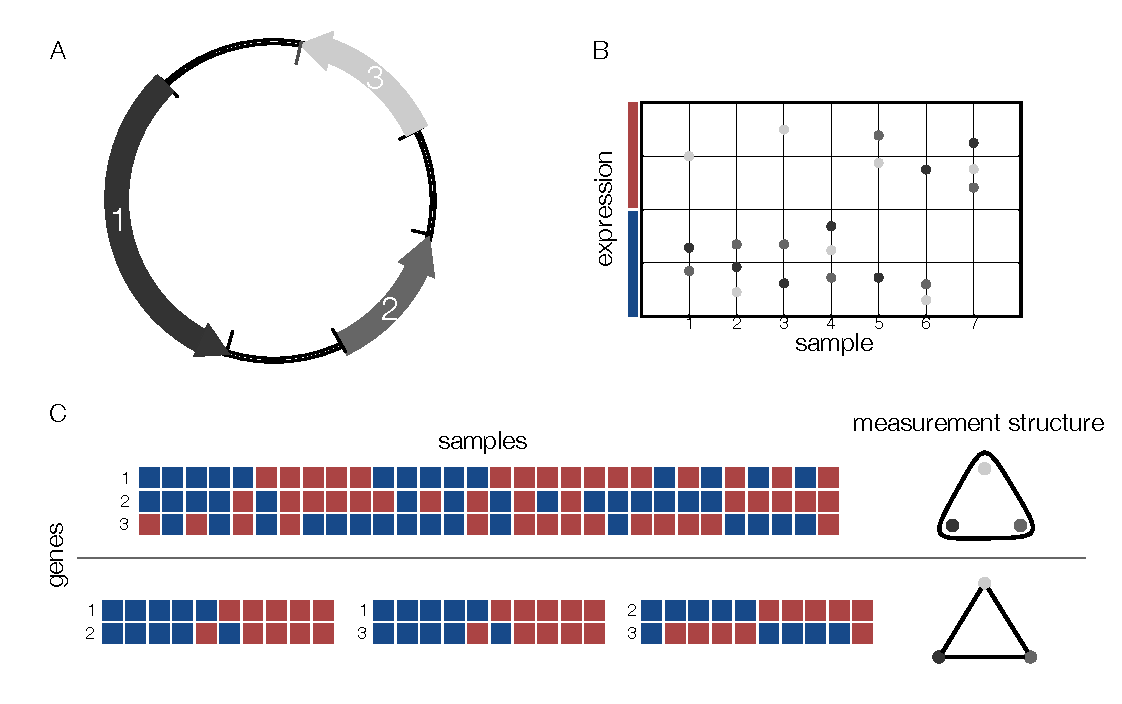
\includegraphics[width=0.9\columnwidth]{fig/figure_expression_concept.pdf}
\caption{{\bf Coarse-graining of gene expression data.} (A) Minimal representation of a small GRN consisting of three genes encoded in a plasmid. (B) Example binary coarse-graining of gene expression data. For each sample a measurement is taken for all three genes. The expression levels are binned into one of two classes represented by the red and blue bars representing relatively high and low expression respectively. (C) Heat map representation of coarse-grained gene expression data under the assumption of two different GRNAs. The samples on top and the associated measurement structure correspond to the case where constraints are placed on all three genes by a single element of the network context (\ref{fig:stochdynscheme} top row). The bottom represents the case where all three pairs of genes are each independently constrained by elements of the network context (\ref{fig:stochdynscheme} bottom row).}
\label{fig:expression_concept}
\end{figure}

\begin{figure}[!ht]
\centering
\noindent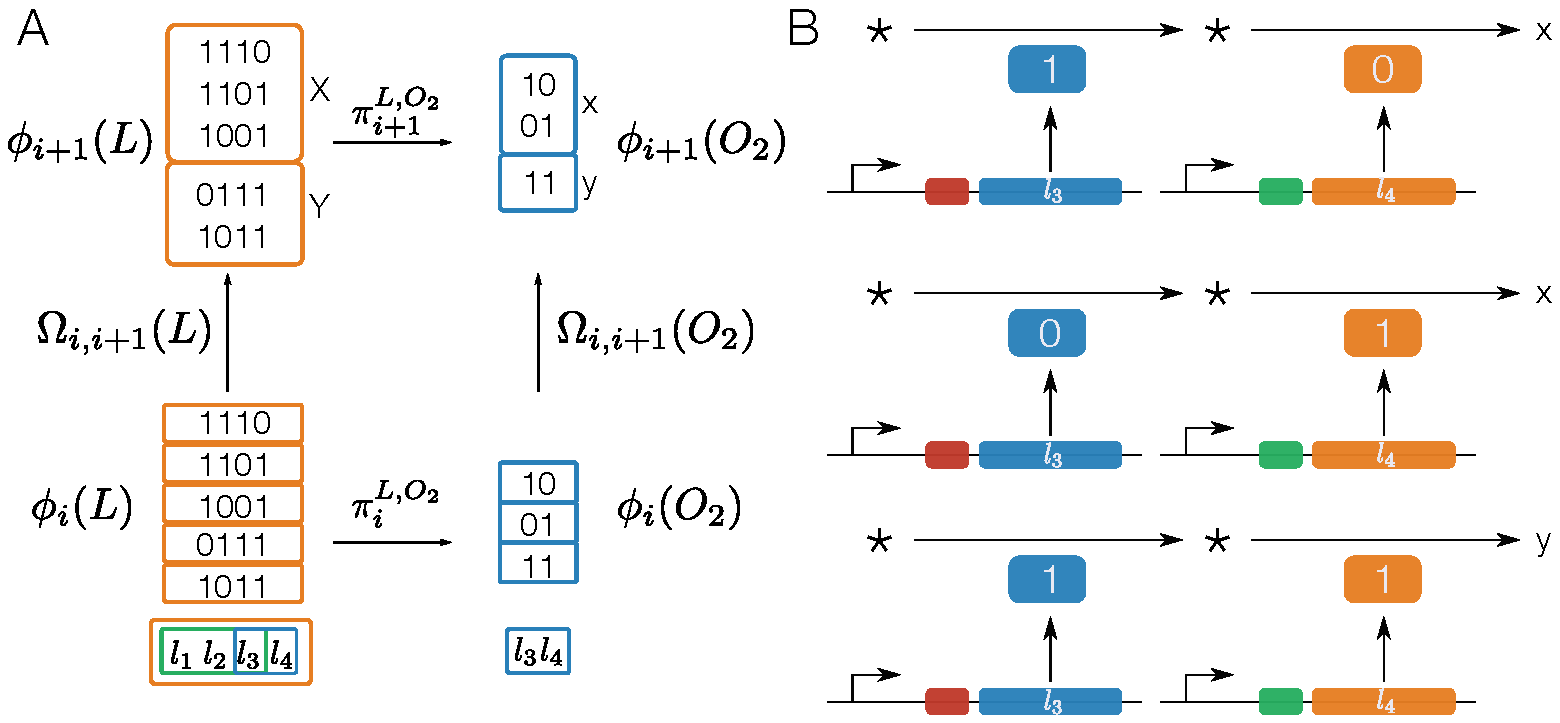
\includegraphics[width=0.9\columnwidth]{fig/phenotypehierarchy.pdf}
\caption{{\bf Example coarse-graining of phenotypes.} (A) \DIFaddbeginFL \DIFaddFL{Consider the example where $L = \{l_1,l_2,l_3,l_4\}$, $\mathcal{G} = \{ O_1, O_2 \}$, $O_1 = \{l_1, l_2, l_3\}$ and $O_2 = \{ l_3, l_4 \}$. }\DIFaddendFL The top left panel shows two higher-level phenotypes $X$ and $Y$. The bottom left corner shows the five different expression states of four genes \DIFdelbeginFL \DIFdelFL{$\{l_1,l_2,l_3,l_4\}$ }\DIFdelendFL \DIFaddbeginFL \DIFaddFL{in $L$ }\DIFaddendFL from which these phenotypes are coarse-grained. The right side shows the respective projections onto genes $\{l_3,l_4\}$. \DIFaddbeginFL \DIFaddFL{The projection maps $\pi_i^{L,O_2}$ and $\pi_{i+1}^{L,O_2}$ are defined in }\refsupp{} \DIFaddFL{\ref{secsupp:coarsegrainingphenotypes}. }\DIFaddendFL (B) The different combinations of expression states of genes $\{l_3,l_4\}$ result in two different phenotypes. If both genes are expressed metabolite $y$ is produced whereas if only one of the two genes is expressed metabolite $x$ is produced. \DIFaddbeginFL \DIFaddFL{The red and green boxes represent arbitrary promoters.}\DIFaddendFL }
\label{fig:phenotypehierarchy}
\end{figure}

\begin{figure}[!ht]
\centering
\noindent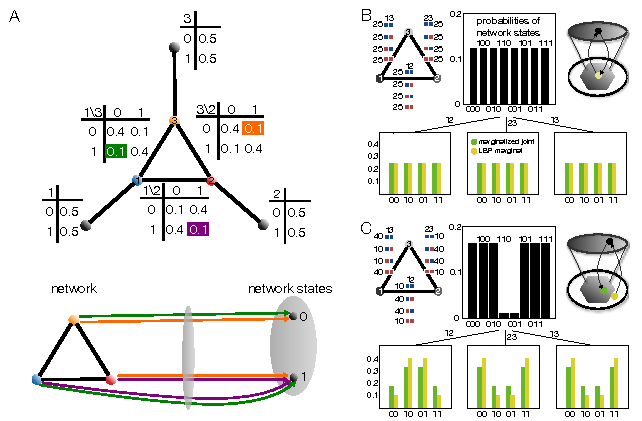
\includegraphics[width=0.9\columnwidth]{fig/inconsistentthreecycle.pdf}
\caption{{\bf Model of inconsistent gene expression data.} (A) An example structured according to \ref{fig:expression_concept}C bottom. The graph contains three nodes each representing one of the genes depicted in \ref{fig:expression_concept}A. The gray node coming from each node is placed next to the node marginal distribution depicted in the associated table. The edge marginal distributions are placed along the edges. The \DIFdelbeginFL \DIFdelFL{colored boxes }\DIFdelendFL \DIFaddbeginFL \DIFaddFL{highlighted table entries }\DIFaddendFL (top) \DIFdelbeginFL \DIFdelFL{are associated to }\DIFdelendFL \DIFaddbeginFL \DIFaddFL{represent }\DIFaddendFL the \DIFaddbeginFL \DIFaddFL{constraint probabilities on the }\DIFaddendFL \gnpm{} represented by the equivalently colored arrows (bottom). The phenotype values derive from the coarse-graining process over gene expression data depicted in \ref{fig:expression_concept}B. (B) Given the model in panel A, the top-left panel represents three hundred samples comprising a data set consistent with a uniform distribution over all \gnpm{}. The top-middle panel represents the joint probability distribution determined via maximum-likelihood estimation with respect to the sufficient statistics (in this case, counts of pairwise observations of genes in states where blue corresponds to 0 and red corresponds to 1) given in the top-left panel. The green bars in the bottom three panels represent the marginalization of this joint distribution according to the structure of the graph. The yellow bars in the bottom three panels represent the ostensible marginal distributions determined via the sum-product algorithm (loopy belief propagation) \cite{Barber2012}. The top-right panel is a schematic where the top gray ellipse represents the space of joint probability distributions on three genes each with two expression states (i.e. $\Delta_7$: the eight-dimensional probability simplex) and the bottom ellipse represents the union of three copies of the four-dimensional probability simplex (i.e. $\Delta_3^{\oplus 3}$), one for each edge in the graph.  For this data, maximum likelihood estimation and loopy belief propagation yield equivalent points in $\Delta_3^{\oplus 3}$\DIFdelbeginFL \DIFdelFL{and therefore the distance separating them is $0$}\DIFdelendFL . (C) Same as B, but with data consistent with \ref{fig:expression_concept}C bottom, which in the limit of a large amount of data would converge to the ostensible node and edge marginal distributions in panel A of this figure. For this data, maximum likelihood estimation and loopy belief propagation yield different points in $\Delta_3^{\oplus 3}$.}
\label{fig:inconsistentthreecycle}
\end{figure}

\begin{figure}[!ht]
\centering
\noindent\DIFdelbeginFL %DIFDELCMD < 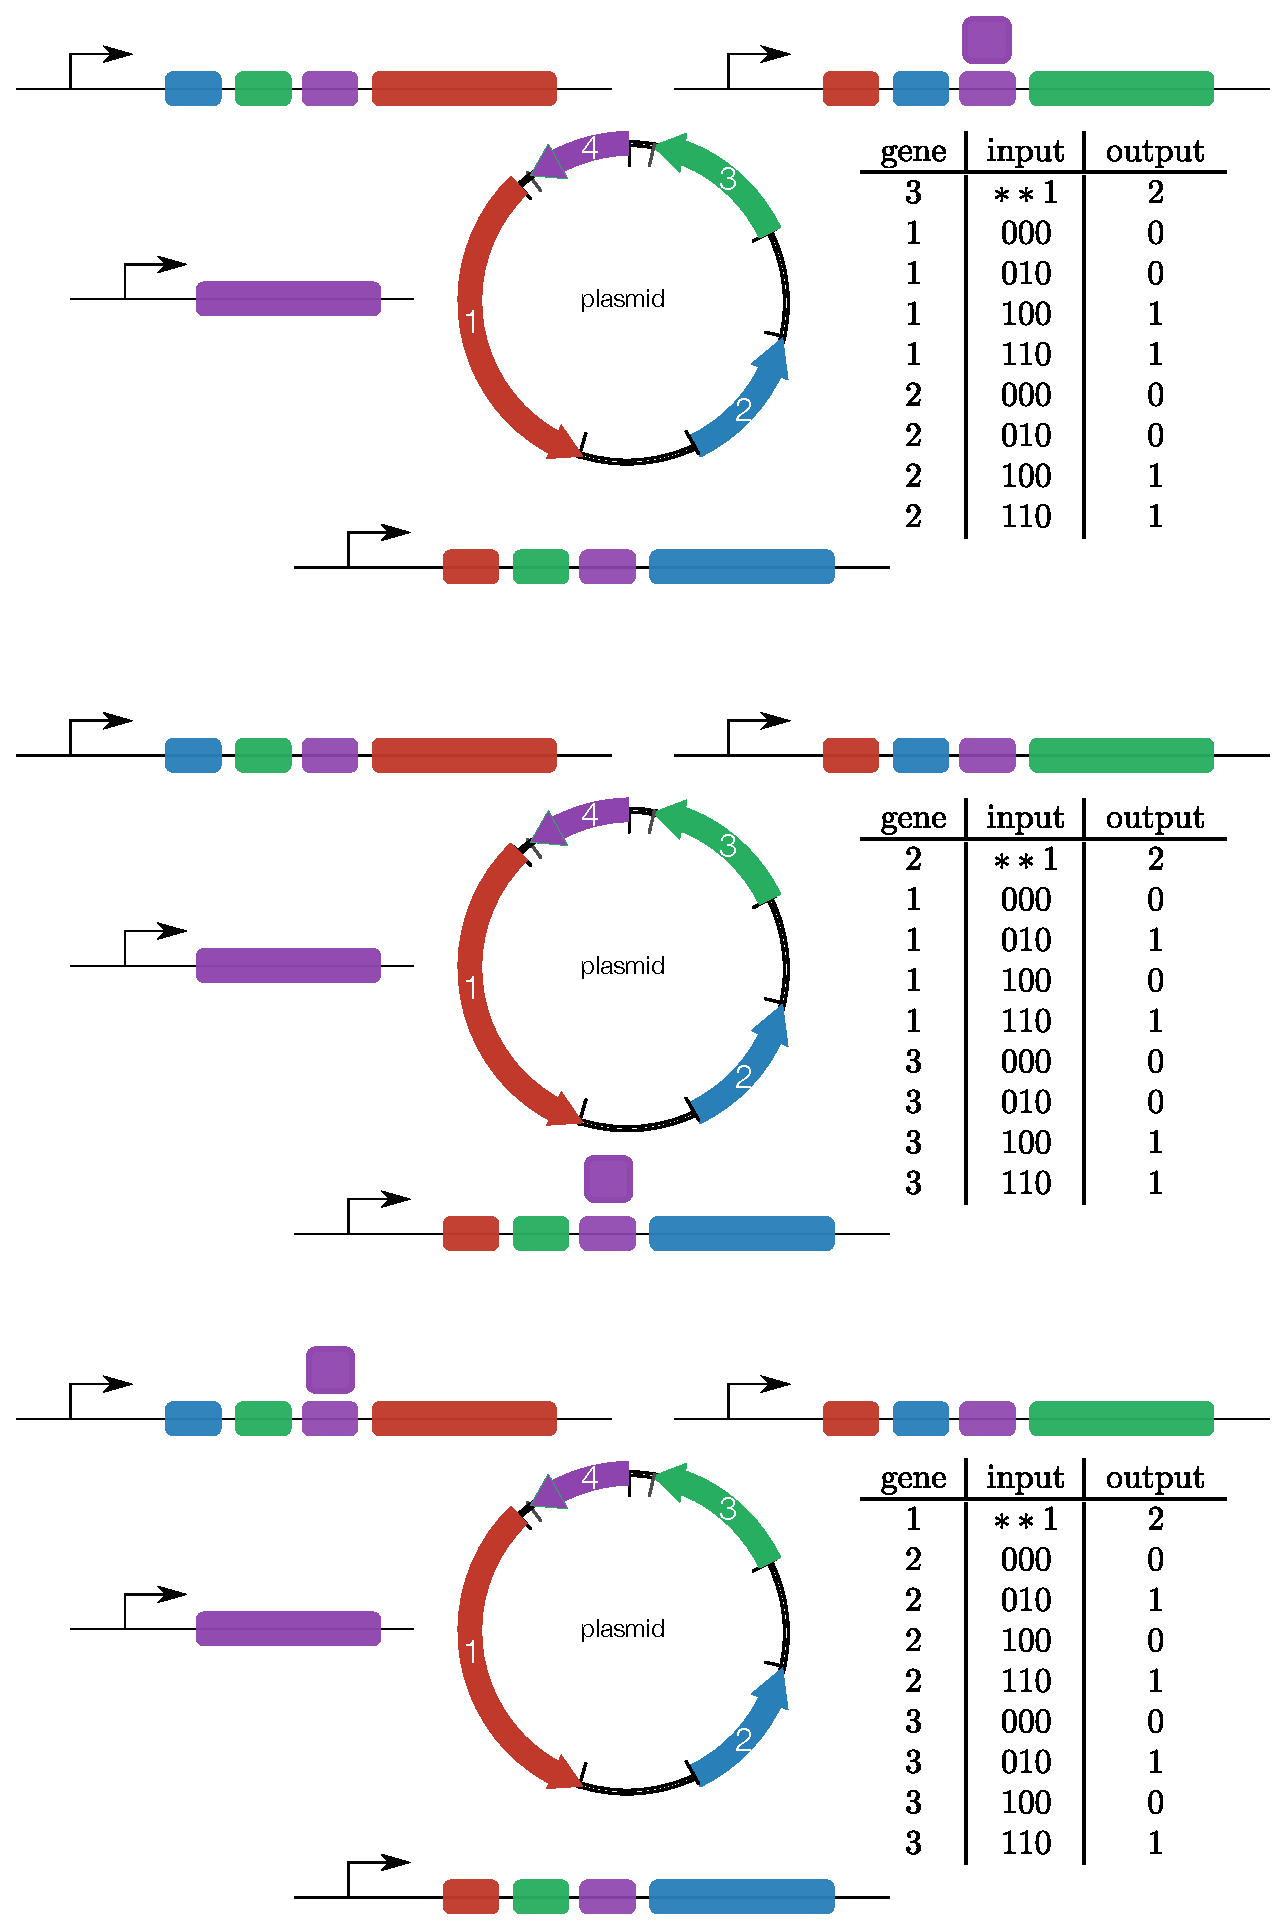
\includegraphics[width=1.0\columnwidth]{fig/condgenescenario.pdf}
%DIFDELCMD < %%%
%DIFDELCMD < \caption{%
{%DIFAUXCMD
%DIFDELCMD < {\bf %%%
\DIFdelFL{Schematic synthetic gene circuit capable of exhibiting apparent inconsistency.}%DIFDELCMD < } %%%
\DIFdelFL{A synthetic gene circuit consisting of four genes possesses one gene (purple) whose product is assumed to be present at low copy number and binds randomly with equal affinity to operator sites existing within the operons of each of the other three genes (red, blue, and green). These latter three genes each possess operator sites for the other two, but do not possess autoregulatory operators. They also each exhibit three states represented by three dynamical modes that may involve intermediates not explicitly represented here \mbox{%DIFAUXCMD
\cite{Cai2008,Dolmetsch1998}
}%DIFAUXCMD
. If the first gene is bound to the operator of another gene, the output is forced into a zero frequency infinite period, or DC, mode (state 2) regardless of the binding state of the other operators. If the first gene is unbound, then the expression state can be switched between low (state 0) and high (state 1) frequency modes depending upon the binding states of other genes as indicated. Note that operators for each of genes one to three are insensitive to the DC mode. Observing pairs of genes one to three and ignoring the state corresponding to the DC mode can lead to apparent inconsistency.}}
%DIFAUXCMD
%DIFDELCMD < \label{fig:condgenescenario}
%DIFDELCMD < \end{figure}
%DIFDELCMD <

%DIFDELCMD < \begin{figure}[!ht]
%DIFDELCMD < \centering
%DIFDELCMD < \noindent%%%
\DIFdelendFL 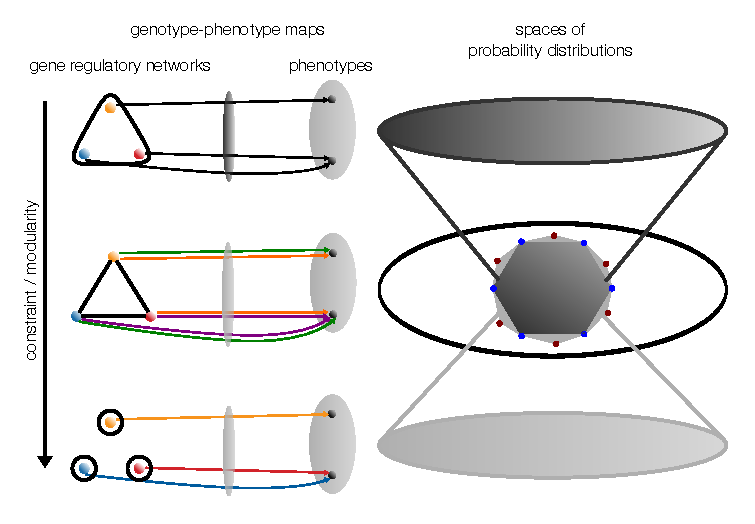
\includegraphics[width=0.9\columnwidth]{fig/conediagram.pdf}
\caption{{\bf Relationship between gene regulatory network models and spaces of probability distributions.} (A) The collection of all possible GRNAs over three genes forms a lattice represented here by its Hasse diagram. An analogous lattice of GRNAs exists for any number of genes. The Hasse diagram shows the manner in which GRNAs are hierarchically related and are thus able to be embedded within one another. (B) Explicit examples of \gnpm{} over three GRNAs from panel A highlighted in green are represented as arrows mapping the genes represented as nodes of the graph underlying the GRNA into the collection of phenotype values determined by the coarse-graining chosen in \ref{fig:expression_concept}B. There is a different collection of possible \gnpm{} depending upon the structure of the GRNA. (C) Each collection of \gnpm{} one representative for each GRNA depicted in panel B is associated to a space of probability distributions defined over it. Moreover, the spaces of probability distributions associated to each graph are related via marginalization maps. The top represents a joint probability distribution which can be marginalized to the middle space which in turn can be marginalized to the bottom space. The light gray polytope in the middle, $\mathbb{L}(\mathcal{G})$, represents the space of distributions consistent with the marginalization map from the middle to the bottom. The dark gray polytope, $\mathbb{M}(\mathcal{G})$, represents the space of probability distributions consistent with marginalization from the top to the middle.}
\label{fig:conediagram}
\end{figure}


\begin{figure}[!ht]
\centering
\noindent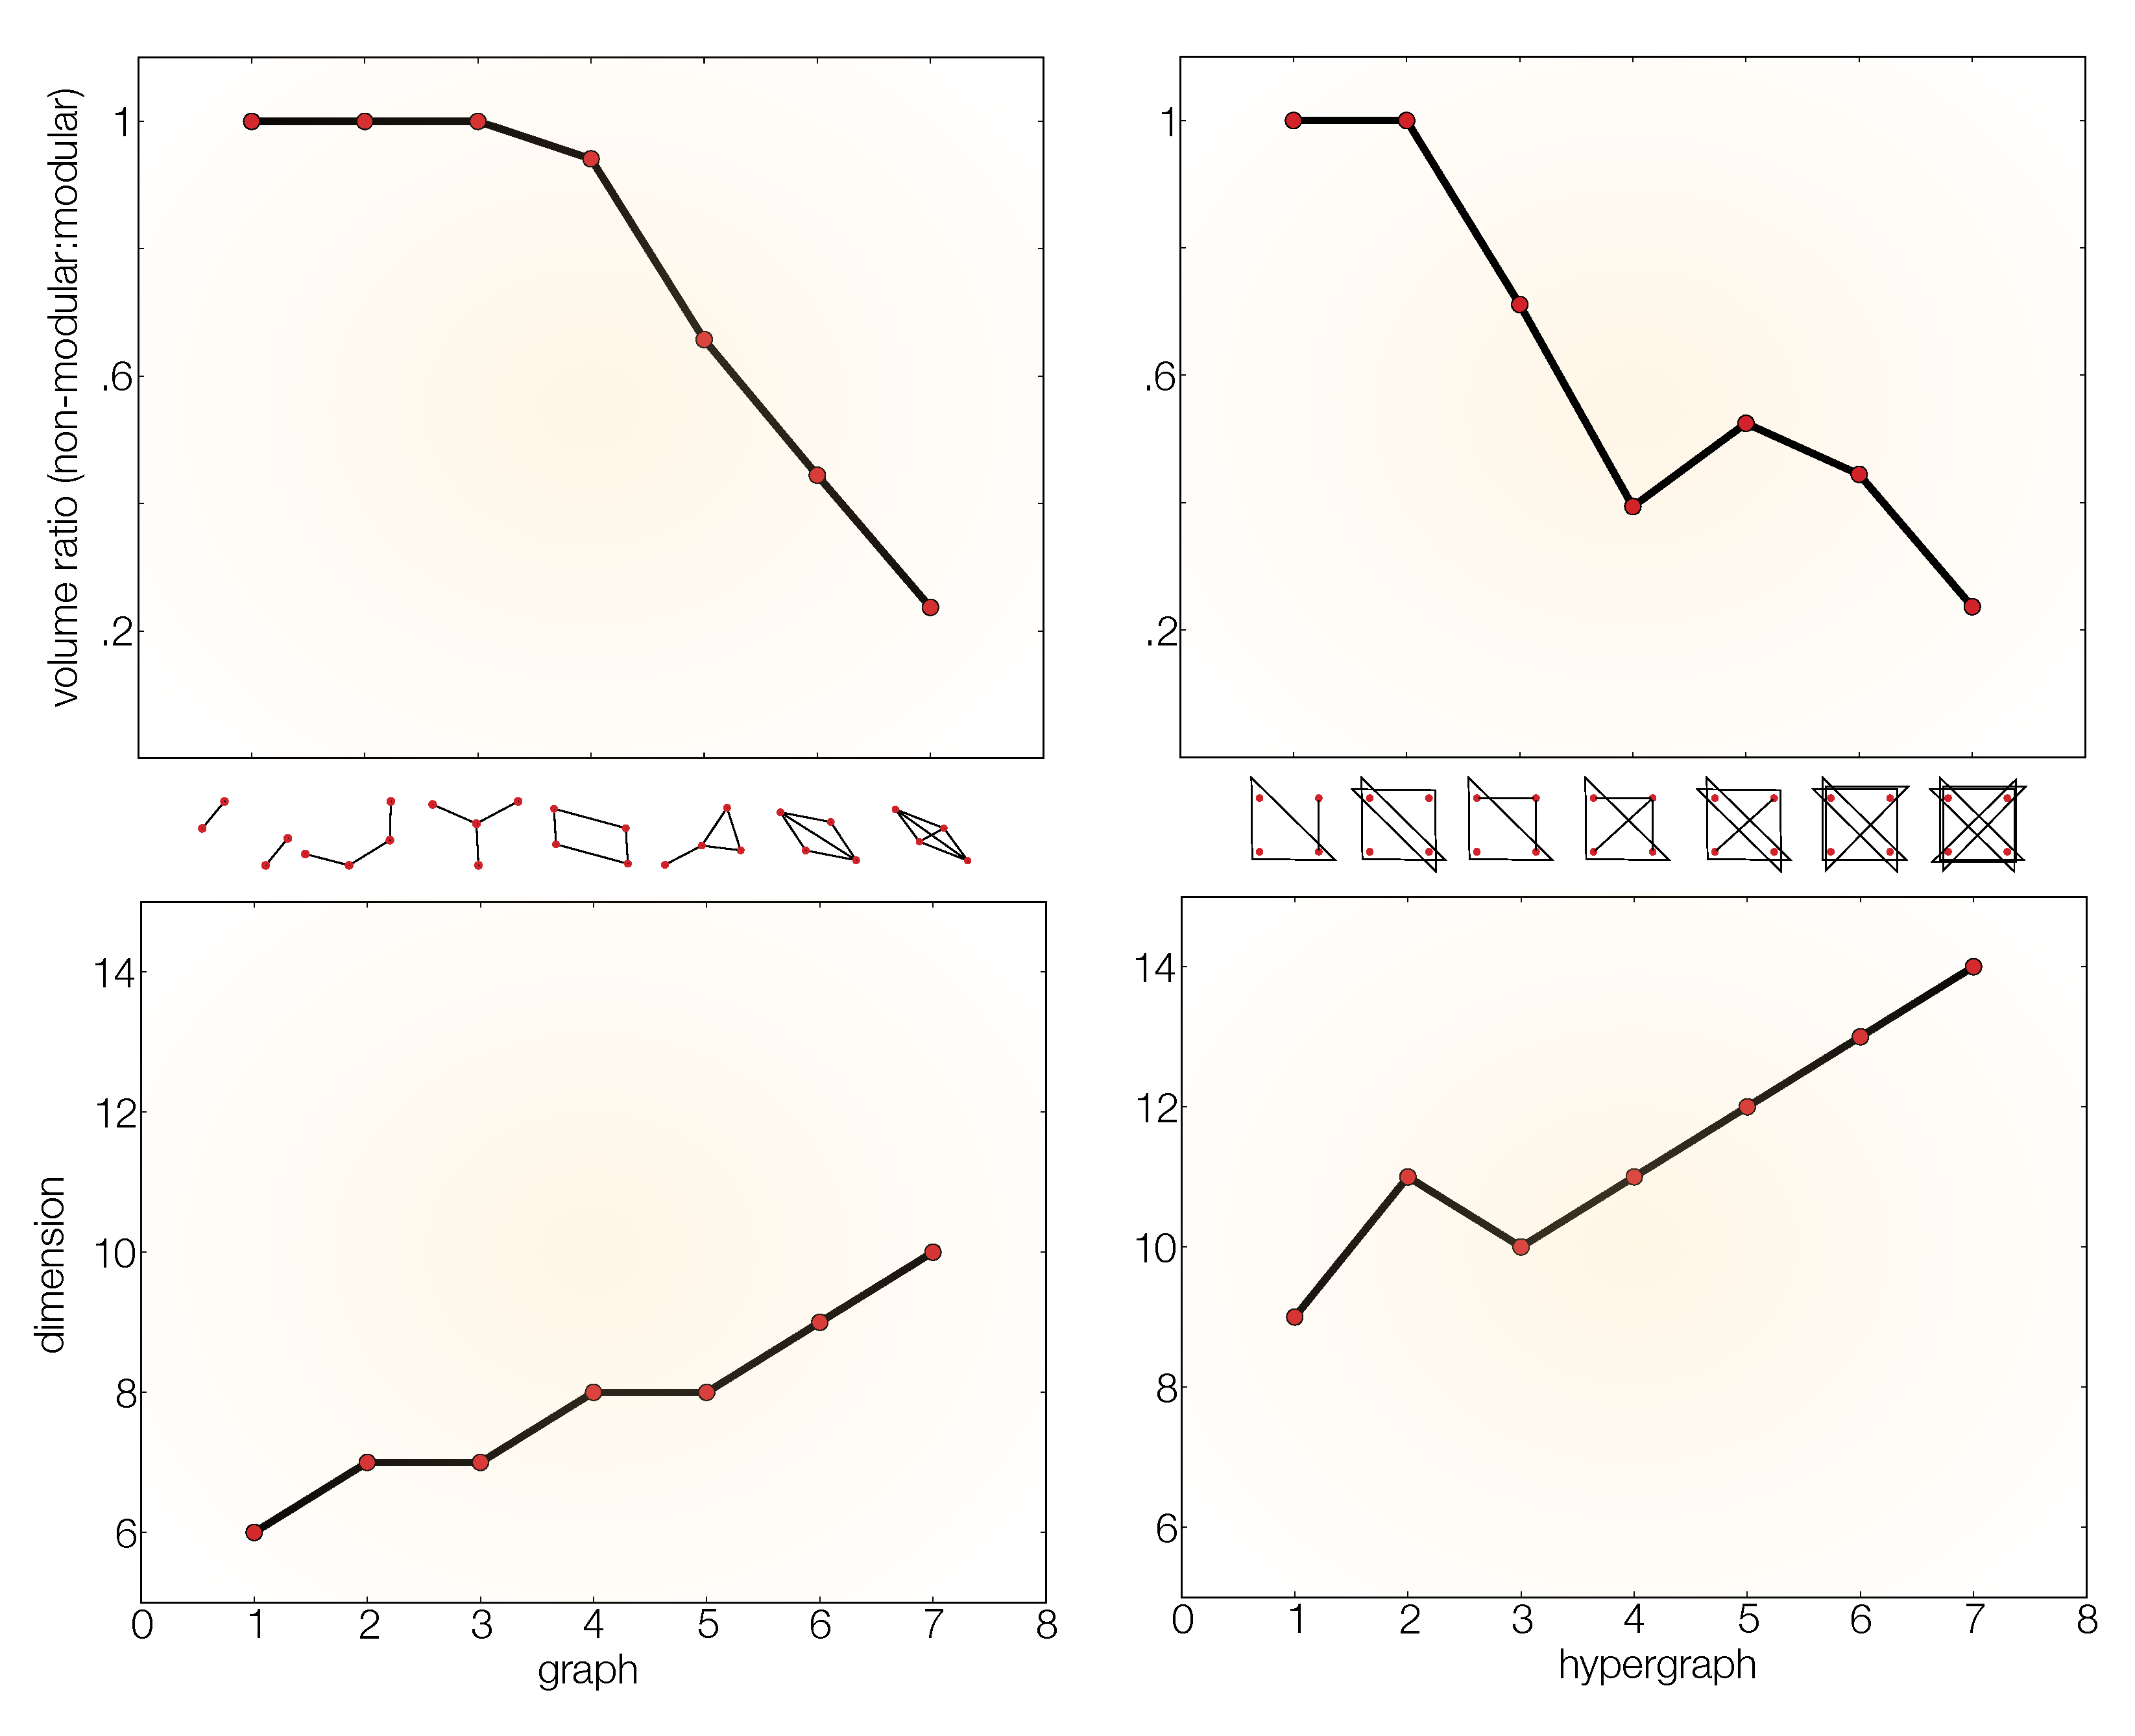
\includegraphics[width=0.9\columnwidth]{fig/figure_graphs_dims_nolines.pdf}
\caption{{\bf Non-modular to modular probability space volume ratio.} (A) and (B) show the ratio $\frac{\text{Vol}(\mathbb{M}(\mathcal{G}))}{\text{Vol}(\mathbb{L}(\mathcal{G}))}$ associated to 2-regular and non-2-regular GRNAs respectively. The (hyper)graph associated to each value of the volume ratio is displayed along the x-axis of each panel. (C) and (D) show the natural dimension of the space of probability distributions associated to $\mathbb{M}(\mathcal{G})$ and $\mathbb{L}(\mathcal{G})$ for each hypergraph.}
\label{fig:ncycvolrat}
\end{figure}

\begin{figure}[!ht]
\centering
\noindent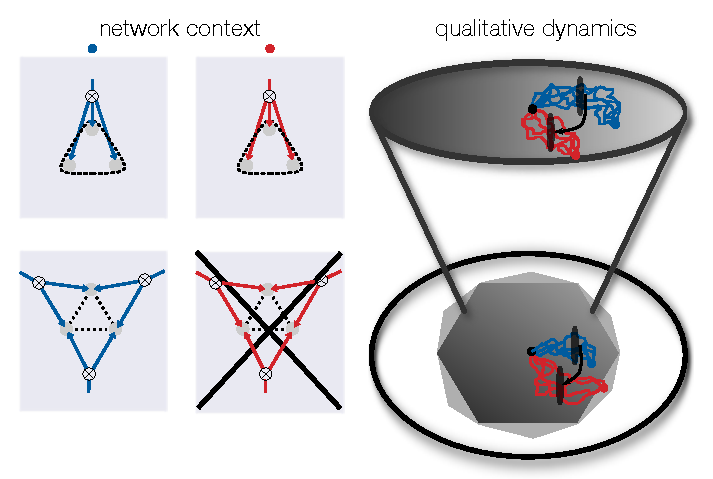
\includegraphics[width=0.9\columnwidth]{fig/stochdynscheme.pdf}
\caption{{\bf Schematic representation of the constraints imposed on stochastic gene expression and evolutionary dynamics by network architecture.} Schematic representation of a potential network context (left) for each of the hypothetical stationary probability distributions associated to the fitness peak established by the blue and red points within the spaces of probability distributions represented on the right. Algebraically, the top one corresponds to $\dist (\expr (L))$ and the bottom to $\dist (\expr (\mathcal{G}))$. Either of the two GRNAs represented on the left are capable of achieving the stationary distribution over \gnpm{} specified by the blue stationary distribution associated to a hypothetical fitness peak. On the other hand, only the GRNA from the top (and not the bottom) is capable of achieving the red stationary distribution representing an alternative potential fitness peak.}
\label{fig:stochdynscheme}
\end{figure}


\FloatBarrier



\pagebreak
\beginsupplement
\setcounter{secnumdepth}{4}
{\noindent\Large\bfseries Supplementary Material}
\makeatletter{}
\DIFdelbegin \section*{\DIFdel{Four cycle example}}
%DIFAUXCMD
\DIFdelend \DIFaddbegin \section{\DIFadd{Functorial formulation of probability distributions over network modules}}\label{secsupp:probabilitydistributionsonnetworks}
\DIFaddend

\DIFdelbegin \DIFdel{For the purposes of this example}\DIFdelend \DIFaddbegin \DIFadd{As stated in \ref{sec:probabilitydistributionsonnetworks}, in addition to the expression state of the whole genome, we usually will be interested in the expression states of portions of the genome that interact either directly or indirectly.  We will represent these portions as subsets of $L$ and their expression states as functions from these subsets to $P$.
}

\DIFadd{The power set of $L$, which we shall denote as $\mathcal{P}(L)$, can be regarded  as a category~\mbox{%DIFAUXCMD
\cite{Lane1998,MacLane1992,Awodey2006,Abramsky2011}
}%DIFAUXCMD
in which the objects are subsets of $L$ and morphisms represent inclusion of a smaller subset into a larger superset (i.e. $O \subseteq O' \Rightarrow O \rightarrow O'$).  Then we will represent our expression states of subsets by the functor $\expr = \mathrm{Hom}(-,P)$.  Specifically, this functor may be described as
}\begin{equation}\DIFadd{\label{eq:gpfunctor}
\begin{split}
\expr \colon (\mathcal{P}(L), \subseteq) &\to \mathbf{Set} \\
O &\mapsto P^O,\\
O \subseteq O' &\mapsto (S \in P^{O'} \mapsto \{e|_O \mid e \in S\}). \end{split}
}\end{equation}
\DIFadd{For example, if we consider the case in which we have two genes $L=\{l_1,l_2\}$ and there are two potential phenotypes, $P=\{0,1\}$, then $\expr$ operates on the lattice of subsets generated by $L$ to give spaces of functions containing the possible }\gnpm{} \DIFadd{as exemplified in \ref{fig:efunctor}.
}

\DIFadd{Next, we introduce extended probability distributions by defining a functor $\mathcal{D}$ that will compose with $\mathcal{E}$ to convert collections of }\gnpm{} \DIFadd{into probability distributions over them.  Given a finite set $S$, define $\dist(S)$ to be the set of all maps from $S$ to the interval $[0,1]$ which satisfy the following two conditions:  For all $d \in \dist(S)$, we have $d(S) \in \{0,1\}$.}\footnote{\DIFadd{Normally, we would only have $d(S) = 1$, but since we want to introduce conditionalization in a coherent way it becomes necessary to admit degenerate distributions where $d(S) = 0$ as well. This simplifies the exposition by not requiring us to worry about dividing by zero and having to introduce special cases when dealing with conditional probabilities and partial functions.  Of course, it also means that we cannot automatically assume that an element of $\dist(S)$ can be normalized without checking this fact but in our examples, this verification will turn out to be routine and trivial.}}  \DIFadd{For all  $d \in \dist(S)$ and all $A, B \subset S$, we have $d(A) + d(B) = d(A \cup B) + d(A \cap B)$.
}

\DIFadd{If $S$ and $S'$ are finite sets, which in our case will usually be sets of }\gnpm{} \DIFadd{given by $\mathcal{E}(O)$}\DIFaddend , \DIFdelbegin \DIFdel{we }\DIFdelend \DIFaddbegin \DIFadd{$d \in \dist(S)$ and $d' \in \dist(S')$ are probability distributions over these spaces, and $f \colon S \to S'$ is a partial function, we will say that $f$ is compatible with $d$ and $d'$ when, for all $X \in \mathrm{img}(f)$, we have
}\begin{equation}\DIFadd{
 d'(X) =
  \begin{cases}
    \frac{d'(\mathrm{img}(f))}{d(\mathrm{dom}(f))}d(f^{-1}(X)) & d(\mathrm{dom}(f)) \neq 0, \\
    0 & d(\mathrm{dom}(f)) = 0.
  \end{cases}
}\end{equation}
\DIFadd{In other words, the map $f$ preserves ratios of probabilities of events.  In the case where $f$ is a partial surjection $(\mathrm{img}(f)=S')$, compatibility completely determines $d'$ in terms of $d$ and thus $\dist$ may be regarded as a functor from the subcategory of sets with partial surjections as morphisms to transformations on probability distributions:
}\begin{equation}\DIFadd{\label{eq:distfunctor}
 d' = \dist(f)(d) =
  \begin{cases}
    X \mapsto \frac{d(f^{-1}(X))}{d(\mathrm{dom}(f))} & d(\mathrm{dom}(f)) \neq 0, \\
    X \mapsto 0 & d(\mathrm{dom}(f)) = 0.
  \end{cases}
}\end{equation}
\DIFadd{Specifically, when $f$ is a total surjection, this map corresponds to marginalization. For example, in the case $f = \expr ( \{ l_1 \} \! \subseteq \! \{ l_1, l_2 \} )$
}\begin{equation}\DIFadd{\label{eq:dfunctorex}
\begin{split}
\dist \big(\expr ( \{ l_1 \} \! \subseteq \! \{ l_1, l_2 \} ) \big) \colon \expr ( \{ l_1 \} \! \subseteq \! \{ l_1, l_2 \} ) &\to \expr ( \{ l_1 \} ), \\
d &\mapsto d',
\end{split}
}\end{equation}
\DIFadd{then
}\begin{equation}\DIFadd{\label{eq:margexample}
d\hspace{.09em}'(\{e^1_0\}) = \dist (f)(d)(\{e^1_0\}) = \frac{d(f^{-1}(\{ e^1_0\}))}{d(\{ e^{12}_{00},e^{12}_{01},e^{12}_{10},e^{12}_{11} \})} = \frac{d(\{ e^{12}_{00},e^{12}_{01}\})}{1} = d( \{ e^{12}_{00} \} ) + d( \{ e^{12}_{01} \} ) = p^{12}_{00} + p^{12}_{01}.
}\end{equation}
\DIFadd{When $f$ is a partial isomorphism, it corresponds to conditionalization. For example, if $f$ is defined such that we condition on gene one being in state zero, $l_1 = 0$,
}\begin{equation}\DIFadd{
f \colon \{ e^{12}_{00} , e^{12}_{01} \} \subset \expr ( \{ l_1, l_2 \} ) \to \{ f(e^{12}_{00}) , f(e^{12}_{01}) \}
}\end{equation}
\DIFadd{then
}\begin{equation}\DIFadd{\label{eq:condexample}
d\hspace{.09em}'(\{ f(e^{12}_{00}) \} ) = \dist (f)(d)( \{ f(e^{12}_{00}) \}) = \frac{d( f^{-1}( \{ f(e^{12}_{00}) \}) )}{d(\{ e^{12}_{00},e^{12}_{01} \})} = \frac{d(\{ e^{12}_{00} \})}{d( \{ e^{12}_{00} \} ) + d( \{ e^{12}_{01} \} )} = \frac{p^{12}_{00}}{p^{12}_{00} + p^{12}_{01}}.
}\end{equation}
\DIFadd{Finally, when $f$ is a general partial surjection, it corresponds to a combination of conditionalization and marginalization.
}

\DIFadd{In order to admit the basic tools of linear algebra for the purpose of calculations regarding relationships between spaces of probability distributions we explain how they embed into linear spaces. By definition, an extended probability distribution $p \in \dist(S)$ is an element of $\mathbb{R}^S$. We denote the inclusion map as
}\begin{equation}\DIFadd{\label{eq:emb}
\rm{emb}(S) : \dist(S) \to \mathbb{R}^S.
}\end{equation}
\DIFadd{Because a convex combination of two probability distributions is again a probability distribution, the image of $\mathrm{emb}(S)$ consists of a convex set and the origin point (corresponding to the degenerate zero distribution).  Furthermore, if $n$ is the number of elements of the set $S$, this convex set works out to be the probability simplex with $n$ vertices, which we denote $\Delta_{n-1}$.  In our example above, $\mathcal{D}(\mathcal{E}(\{l_1,l_2\}))$ is the tetrahedron $\Delta_3$. Since any vector $v \in \mathbb{R}^S$ may be written as $v = c_{+} p_{+} - c_{-} p_{-}$ where $c_{+}, c_{-} \in [0,\infty)$ and $p_{+}$ and $p_{-}$ are probability distributions, the image of $\mathrm{emb}(S)$ spans the vector space $\mathbb{R}^S$.  For purposes of later reference, note that, if $f \colon S \to S'$ is a partial surjection, then $\mathcal{D}$ extends to a fractional linear map, as in \ref{eq:condexample}, from $\mathbb{R}^S$ to $\mathbb{R}^{S'}$ and that, in the special case where $f$ is a total surjection, as in \ref{eq:margexample}, it is in fact a linear map.
}

\section{\DIFadd{Precise formulation of coarse-graining phenotypes}}\label{secsupp:coarsegrainingphenotypes}

\DIFadd{Recall from \ref{sec:coarsegrainingphenotypes} that for each set of genes $O \in \mathcal{P}(L)$, let $\phi_i (O)$ be the set of phenotype values at level $i$, which can be determined from the expression levels of genes in $O$.  When $O_1 \subseteq O_2 \in \mathcal{P}(L)$, we have a restriction map $\pi_i^{O_2 O_1} \colon \phi_i(O_2) \to \phi_i(O_1)$.  These maps satisfy the consistency conditions that $\pi_i^{OO}$ is the identity map and that $\pi_i^{O_3 O_2} \circ \pi_i^{O_2 O_1} = \pi_i^{O_3 O_1}$, i.e. $\pi_i$ is a functor on $(\mathcal{P}(L), \subseteq)$.  As stated earlier, we set $\phi_1 (O) = P^O$ and $\pi_1^{O_2 O_1}$ to be the restriction map from $P^{O_2}$ to $P^{O_1}$.  If $i \le j$, let $\Omega_{ij}(O) : \phi_i(O) \to \phi_j(O)$ be the coarse-graining map which describes how higher level phenotypes are determined from lower level phenotypes.  These maps are all surjections and, for consistency, we will require the following conditions:
}\begin{enumerate}
\item \DIFadd{$\Omega_{ij}(O) \circ \Omega_{jk}(O) = \Omega_{ik}(O)$ whenever $i \le j \le k$.
}\item \DIFadd{$\Omega_{ii}(O)$ is the identity map on $\phi_i (O)$.
}\item \DIFadd{If $O_1 \subseteq O_2 \in \mathcal{P}(L)$ and $i > j$, then $\Omega_{ij}(O_1) \circ \pi_i^{O_2 O_1} = \pi_j^{O_2 O_1} \circ \Omega_{ij}(O_2)$
}\end{enumerate}
\DIFadd{In other words, $\Omega$ must be suitably functorial in both of its arguments.
}

\DIFadd{Since the map $\Omega_{1i}(O)$ is a surjection from $P^O$ onto $\phi_i(O)$, we can use it to map our probabilistic structures to $\phi_i(O)$.  Set $\mathcal{E}_i = \Omega_{1i}(O)^{-1} \circ \mathcal{E}$ and $\dist_i = \Omega_{1i}(O)^{-1} \circ \dist$.  Then we end up with the overall relationships summarized in \ref{fig:abstractroadmap}. As a consequence of the consistency conditions the coarse-graining maps $\phi$ and $\Omega$, there is a natural transformation between the functors $\expr_i$ and $\expr_{i+1}$ implying that the following diagram commutes
}$$\DIFadd{
\xymatrix{
\expr_{i+1}(O_1) \ar[r]^{\expr_{i+1}(\subseteq)} \ar[d]_{t_{O_1}} & \expr_{i+1}(O_2) \ar[d]^{t_{O_2}} \\
\expr_{i}(O_1) \ar[r]^{\expr_{i}(\subseteq)} & \expr_{i}(O_2) }
}$$
\DIFadd{for any $O_2 \subseteq O_1$.
}

\section{\DIFadd{Sheaf-theoretic formulation of compatibility of distributions on }\gnpm{}}\label{secsupp:compatibilityofgpms}
\DIFadd{Recall from \ref{sec:compatibilityofgpms} that given a covering of the space of genes $\mathcal{G}$, a compatible family for $\mathcal{G}$ with respect to $\mathcal{D} \circ \mathcal{E}$ is given by a family of distributions $\{d_O \in \dist (\mathcal{E}(O)) | O \in \mathcal{G}\}$ such that for all $O, O' \in \mathcal{G}$
}\begin{eqnarray}\DIFadd{
d_O|O \cap O' = d_{O'}|O \cap O'.
}\end{eqnarray}
\DIFadd{This first set of conditions is later referred to as local consistency. These conditions mean that any two distributions $d_O$ and $d_{O'}$ in the }\emph{\DIFadd{compatible family}} \DIFadd{of distributions marginalize to the same disribution over the intersection of $O$ with $O'$.
}

\DIFadd{If, moreover, this first condition implies the existence of $d \in \mathcal{D}( \mathcal{E}(L))$ such that $d|O = d_O$ for all $O \in \mathcal{G}$ then the system is said to satisfy the global consistency condition.  This latter condition is also referred to as the }\emph{\DIFadd{sheaf condition}}\DIFadd{.  $\mathcal{E}$ alone turns out to be a sheaf because it satisfies the analogous conditions: for $\{e_O \in \mathcal{E}(O) | O \in \mathcal{G}\}$ such that $e_{O_{1}} | O_1 \cap O_2 = e_{O_{2}} | O_1 \cap O_2$ there exists $e \in \mathcal{E}(\cup_{O \in \mathcal{G}} O)$ such that $e_O = e|O$ for all $O \in \mathcal{G}$.  However, for $\dist \circ \mathcal{E}$ the sheaf condition is not automatically satisfied and it only defines a presheaf.  We will now examine the situation more closely to determine under what circumstances global consistency holds.
}

\DIFadd{For a cover of the genotype space, $\mathcal{G}$, we can construct a matrix, $\mathbf{G}$, representing the relationship, $R = \coprod_{O \in \mathcal{G}} \mathcal{E}(O \subset L) \subseteq \mathcal{E}(L) \times \expr (\mathcal{G})$, between }\gnpm{} \DIFadd{having as domain particular gene regulatory network modules given by the $O \in \mathcal{G}$ and those global }\gnpm{} \DIFadd{defined on $L$. We would like to construct the matrix representation of $\mathbf{G}$. In the first factor, $\mathcal{E}(L) = P^L = \{e^{L}_{\vec{j}} | \vec{j} \in P^{|L|}\}$.
For the second factor, $ \mathcal{E}(\mathcal{G}) = \coprod_{O \in \mathcal{G}} \mathcal{E}(O) = \{e^O_{\vec{i}} | O \in \mathcal{G}, \vec{i} \in P^{|O|} \}$.
 So we have two sets of maps, one defined on $P^L$ and the other defined on $\mathcal{E}(O) = P^O$ for each $O \in \mathcal{G}$. This yields the method of specifying the intended relationship that defines $\mathbf{G}$ for all $e^O_{\vec{i}} \in \mathcal{E}(\mathcal{G})$ and $e^{L}_{\vec{j}} \in \mathcal{E}(L)$ given in \ref{eq:margmat}.
This matrix can be viewed as an operator acting via matrix multiplication on distributions
}\begin{eqnarray*}\DIFadd{
\mathbf{G} \colon \mathcal{D}(\mathcal{E}(L)) }&\DIFadd{\rightarrow}& \DIFadd{\mathcal{D}( \mathcal{E}(\mathcal{G})),}\\
\DIFadd{d }&\DIFadd{\mapsto}& \DIFadd{\coprod_{O \in \mathcal{G}} d|O,
}\end{eqnarray*}
\DIFadd{and thereby taking a global distribution, $\dist (\mathcal{E}(L))$, defined on }\gnpm{} \DIFadd{whose domain is the full set of genes $L$ into the local distributions, $\dist (\mathcal{E}(\mathcal{G}))$, that are defined relative to gene regulatory network modules contained in a covering of the genotype space $\mathcal{G}$. $\mathbf{G}$ provides a way of determining the distributions on }\gnpm{} \DIFadd{for a given context (i.e. $\coprod_{O \in \mathcal{G}} d|O$) that can be derived from distributions (i.e. $\mathcal{D} ( \mathcal{E}(L) )$) defined on the global }\gnpm{} \DIFadd{(i.e. $\mathcal{E}(L)$ as opposed to $\mathcal{E}(O)$).
}

\DIFadd{Combining the marginalization matrix $\mathbf{G}$ with the maps previously defined in \ref{eq:emb} the following diagram demonstrates the relationships between the spaces of probability distributions and the linear spaces in which they are embedded
}

\begin{equation*}
\xymatrix{\DIFadd{
 \mathbb{R}^{\mathcal{E}(L)} \ar[r]^{\mathbf{G}} &
   \mathbb{R}^{\mathcal{E}(\mathcal{G})} \\
 \dist (\mathcal{E}(L)) \ar[r]^{\mathbf{G}} \ar@{^{(}->}[u]^{emb_{\mathcal{E}(L)}}& \ar@{^{(}->}[u]_{emb_{\mathcal{E}(\mathcal{G})}}
  \dist (\mathcal{E}(\mathcal{G}))
  }
}
\end{equation*}
\DIFadd{The locally, $\mathbb{L}(\mathcal{G})$, and globally, $\mathbb{M}(\mathcal{G})$, consistent polytopes embedded within $\mathbb{R}^{\mathcal{E}(\mathcal{G})}$ correspond to the spaces of probability distributions satisfying the local and global consistency conditions described above. The globally consistent polytope is a subspace of the locally consistent one. This is because an ostensible inverse to $\mathbf{G}$ is underdetermined and can only be estimated in general (most commonly using the maximum entropy principle). In terms of the diagram $\mathbb{M}(\mathcal{G})$ is given by $\mathbf{G}(emb_{\mathcal{E}(L)}(\mathcal{D}(\mathcal{E}(L))))$ and $\mathbb{L}(\mathcal{G})$ is given by $emb_{\mathcal{E}(\mathcal{G})}(\mathcal{D}(\mathcal{E}(\mathcal{G}))) \cap \mathbf{G}(\mathbb{R}^{\mathcal{E}(L)})$, where
}\begin{eqnarray}\DIFadd{
emb_{\mathcal{E}(\mathcal{G})}(\mathcal{D}(\mathcal{E}(\mathcal{G}))) }&\DIFadd{=}& \DIFadd{\left\{ p^{O}_{\vec{i}} \; \bigg| \; (\forall\, O \in \mathcal{G}) \; (\forall\, \vec{i} \in P^{|O|}) \;\; p^O_{\vec{i}} \geq 0, \; (\forall\, O \in \mathcal{G}) \sum_{\vec{i} \in P^{|O|}} p^{O}_{\vec{i}} = 1 \right\}, \label{eq:embdeg}}\\
\DIFadd{emb_{\mathcal{E}(L)}(\mathcal{D}(\mathcal{E}(L))) }&\DIFadd{=}& \DIFadd{\left\{ p^L_{\vec{i}} \; \bigg| \; (\forall\, \vec{i} \in P^{|L|}) \; p^L_{\vec{i}} \geq 0, \; \sum_{\vec{i} \in P^{|L|}} p^L_{\vec{i}} = 1 \right\}. \label{eq:embdel}
}\end{eqnarray}
\DIFadd{If the embedding into linear spaces is to be considered explicitly, then \ref{eq:embdeg} and \ref{eq:embdel} can be substituted for $\dist{}(\expr{}(\mathcal{G}))$ and $\dist{}(\expr{}(L))$ in \ref{eq:localpolytope} and \ref{eq:globalpolytope}.
}

\subsection{\DIFadd{Example of apparent satisfaction of unsatisfiable constraints}}\label{secsupp:apparentinconsistency}
\DIFadd{The inequalities defining $\mathbb{M}(\mathcal{G})$ were derived under the assumption that the two-element probabilities were obtained by mariginalizing a three-element distribution.  If some other procedure, such as conditionalization, is used to obtain them instead, these inequalities need not apply. For example, suppose now that $L = \{l_1,l_2,l_3 \}$, $P = \{0,1,2\}$, $\mathcal{G} = \{\{l_1,l_2\},\{l_2,l_3\},\{l_3,l_1\}\}$ where we have simply added an element to $P$ relative to the example described above. In the previous example the marginal maps were given by $\dist (\expr (O \subset L))$ with one for each $O \in \mathcal{G}$. If we combine these marginal maps with conditioning on one out of the three genes being in state two and each of the other two being in states zero or one, then we have instead $\dist (\pi_1), \dist (\pi_2), \dist (\pi_3)$ where $\pi_1 = \expr (\{l_1,l_2\} \subset L)|\{ e^{123}_{ij2} \mid i,j \in \{ 0,1 \} \},\; \pi_2 = \expr (\{l_2,l_3\} \subset L)|\{ e^{123}_{2ij} \mid i,j \in \{ 0,1 \} \},\; \pi_3 = \expr (\{l_3,l_1\} \subset L)|\{ e^{123}_{i2j} \mid i,j \in \{ 0,1 \} \}$. In this case, if we have the following assignment of probabilities for a distribution $d$
}
\begin{equation}\DIFadd{\label{eq:condprobs}
\begin{aligned}
p^{123}_{002} }&\DIFadd{= 1/30 }& \DIFadd{p^{123}_{020} }&\DIFadd{= 2/15 }& \DIFadd{p^{123}_{200} }&\DIFadd{= 2/15}\\
\DIFadd{p^{123}_{012} }&\DIFadd{= 2/15 }& \DIFadd{p^{123}_{021} }&\DIFadd{= 1/30 }& \DIFadd{p^{123}_{201} }&\DIFadd{= 1/30}\\
\DIFadd{p^{123}_{102} }&\DIFadd{= 2/15 }& \DIFadd{p^{123}_{120} }&\DIFadd{= 1/30 }& \DIFadd{p^{123}_{210} }&\DIFadd{= 1/30}\\
\DIFadd{p^{123}_{112} }&\DIFadd{= 1/30 }& \DIFadd{p^{123}_{121} }&\DIFadd{= 2/15 }& \DIFadd{p^{123}_{211} }&\DIFadd{= 2/15}
\end{aligned}
\end{equation}
\DIFadd{with all other probabilities being zero, then $\dist (\pi_1)(d), \dist (\pi_2)(d), \dist (\pi_3)(d)$ are equivalent to the probability tables in \ref{fig:inconsistentthreecycle}A, which as shown in \ref{sec:inconsistency}, could not be achieved by marginalization alone. For example, given that $dom(\pi_1) = \{ e^{123}_{002}, e^{123}_{012}, e^{123}_{102}, e^{123}_{112} \}$ then $d(dom(\pi_1)) = \frac{1}{30} + \frac{2}{30} + \frac{2}{30} + \frac{1}{30} = \frac{1}{3}$. Substituting this factor and the fact that ${\pi_1}^{-1}(e^{12}_{ij}) = e^{123}_{ij2}$ into \ref{eq:distfunctor}
}$$\DIFadd{
p^{12}_{ij} = \dist (\pi_1)(d)(e^{12}_{ij}) = \frac{d({\pi_1}^{-1}(e^{12}_{ij}))}{d(dom(\pi_1))} = 3 p^{123}_{ij2},
}$$
\DIFadd{then renormalizes probabilities resulting in $p^{12}_{00} = 0.1, p^{12}_{01} = 0.4, p^{12}_{10} = 0.4, p^{12}_{11} = 0.1$ along with the analogs for $p^{23}_{ij}$ and $p^{13}_{ij}$, which are precisely equivalent to what appears in \ref{fig:inconsistentthreecycle}A as suggested above.
}

\DIFadd{If constraints consistent with those of \ref{fig:inconsistentthreecycle}A are placed on the given network, either the network must add another gene in order to satisfy them directly or the network context imposing those constraints must coarse-grain the network in a suitable way. In what follows, we argue that the former is much more plausible than the latter. This ultimately suggests conditions in which cycle breakage via gene duplication may be selected for to relieve inconsistent constraints that can arise when cycles are present.
}


\section{\DIFadd{Example volume ratio computation for the four-cycle GRNA}}\label{secsupp:fourcycleexample}

\DIFadd{For the purposes of this example, we }\DIFaddend take the full set of genes to be $L = \{ l_1,l_2,l_3,l_4 \}$. Consider the case in which each of the gene regulatory network modules under consideration has two genes and we specify the covering of the genotype space given by $\mathcal{G} = \{\{l_1,l_2 \},\{l_1,l_4 \},\{l_3,l_2\},\{l_3,l_4\} \}$.  We will compute $\mathbb{L}(\mathcal{G})$ using the same method which was used for the example of three genes.  By analogy with \ref{eq:localconsistencythreegenes}, the local consistency conditions now are as follows:
\begin{equation}
\begin{aligned}\label{eq:pparsys}
p^1_0 &= p^{12}_{00} + p^{12}_{01} = p^{14}_{00} + p^{14}_{01}, &
p^1_1 &= p^{12}_{10} + p^{12}_{11} = p^{14}_{10} + p^{14}_{11},\\
p^3_0 &= p^{32}_{00} + p^{32}_{01} = p^{34}_{00} + p^{34}_{01},&
p^3_1 &= p^{32}_{10} + p^{32}_{11} = p^{34}_{11} + p^{34}_{11},\\
p^2_0 &= p^{12}_{00} + p^{12}_{10} = p^{32}_{00} + p^{32}_{10},&
p^2_1 &= p^{12}_{01} + p^{12}_{11} = p^{32}_{01} + p^{32}_{11},\\
p^4_0 &= p^{14}_{00} + p^{14}_{10} = p^{34}_{00} + p^{34}_{10},&
p^4_1 &= p^{14}_{01} + p^{14}_{11} = p^{34}_{01} + p^{34}_{11}.
\end{aligned}
\end{equation}
Likewise, the equations determined by the conditions $v = \mathbf{G}(x)$ which are analogous to the matrix $\mathbf{G}$ in \ref{fig:efunctor}B are now
\begin{equation}
\begin{aligned}\label{eq:globsys}
p^{12}_{00} &= p^{1234}_{0000} + p^{1234}_{0010} + p^{1234}_{0001} + p^{1234}_{0011} &
p^{12}_{10} &= p^{1234}_{1000} + p^{1234}_{1010} + p^{1234}_{1001} + p^{1234}_{1011} \\
p^{12}_{01} &= p^{1234}_{0100} + p^{1234}_{0110} + p^{1234}_{0101} + p^{1234}_{0111} &
p^{12}_{11} &= p^{1234}_{1100} + p^{1234}_{1110} + p^{1234}_{1101} + p^{1234}_{1111} \\
p^{14}_{00} &= p^{1234}_{0000} + p^{1234}_{0001} + p^{1234}_{1000} + p^{1234}_{1001} &
p^{14}_{10} &= p^{1234}_{0010} + p^{1234}_{0011} + p^{1234}_{1010} + p^{1234}_{1011} \\
p^{14}_{01} &= p^{1234}_{0100} + p^{1234}_{0101} + p^{1234}_{1100} + p^{1234}_{1101} &
p^{14}_{11} &= p^{1234}_{0110} + p^{1234}_{0111} + p^{1234}_{1110} + p^{1234}_{1111} \\
p^{32}_{00} &= p^{1234}_{0000} + p^{1234}_{0010} + p^{1234}_{0100} + p^{1234}_{0110} &
p^{32}_{10} &= p^{1234}_{1000} + p^{1234}_{1010} + p^{1234}_{1100} + p^{1234}_{1110} \\
p^{32}_{01} &= p^{1234}_{0001} + p^{1234}_{0011} + p^{1234}_{0101} + p^{1234}_{0111} &
p^{32}_{11} &= p^{1234}_{1001} + p^{1234}_{1011} + p^{1234}_{1101} + p^{1234}_{1111}\\
p^{34}_{00} &= p^{1234}_{0000} + p^{1234}_{1000} + p^{1234}_{0100} + p^{1234}_{1100} &
p^{34}_{10} &= p^{1234}_{0010} + p^{1234}_{1010} + p^{1234}_{0110} + p^{1234}_{1110} \\
p^{34}_{01} &= p^{1234}_{0001} + p^{1234}_{1001} + p^{1234}_{0101} + p^{1234}_{1101} &
p^{34}_{11} &= p^{1234}_{0011} + p^{1234}_{1011} + p^{1234}_{0111} + p^{1234}_{1111},
\end{aligned}
\end{equation}
which are displayed in matrix form in \ref{tab:logmat222}.

Rather than proceeding to compute $\mathbb{L}(\mathcal{G})$ using elimination of inequalities as before, we will instead make use of the fact that the extremal points of $\mathbb{L}(\mathcal{G})$ happen to be the extremal points of $\mathbb{L}(\mathcal{G})$ with integer coordinates.  This is the approach which was used to compute the volume ratios shown in \ref{fig:ncycvolrat}.  More specifically, those computations were done using a computer program based on the following algorithm which is available via a virtual machine that can be reconstructed using the instructions available on \href{https://github.com/cameronraysmith/sep}{github}:

\begin{enumerate}
\item Compute (a basis for) the cokernel of $\mathbf{G}$. The cokernel gives the obstructions to the system $\mathbf{G}\mathbf{X}=\mathbf{V}$ having a solution. In order to eliminate these obstructions constraints must be imposed on $\mathbb{R}^{\mathcal{E}(\mathcal{G})}$ and these constraints are given precisely via annihilating the cokernel.
\item Use the constraints on $\mathbb{R}^{\mathcal{E}(\mathcal{G})}$ from step 1 necessary for the system $\mathbf{G}\mathbf{X}=\mathbf{V}$ to have a solution to eliminate variables from the system of inequalities $\mathbf{V} \geq 0$ giving a half-space representation or H-representation of the polytope $\mathbb{L}(\mathcal{G})$. This can be used to compute $\text{Vol}(\mathbb{L}(\mathcal{G}))$.
\item Compute the vertices of $\mathbb{L}(\mathcal{G})$ from the H-representation determined in step 2 giving a vertex representation or V-representation of $\mathbb{L}(\mathcal{G})$.
\item Filter the non-integer rational vertices from the collection computed in step 3 to produce a corresponding V-representation of $\mathbb{M}(\mathcal{G})$ \cite{Wainwright2007} proposition 8.3.
\item Compute $\text{Vol}(\mathbb{M}(\mathcal{G}))$ from the V-represention of $\mathbb{M}(\mathcal{G})$.
\end{enumerate}

For standard computations on polytopes, we make use of the standard algorithms incorporated by the polymake project \cite{Gawrilow2000}. In some cases, the volume computation is too costly to perform exactly. In those cases we use the approximation given in \cite{Cousins}.  We now return to our example of four genes $\mathcal{G} = \{\{l_1,l_2 \},\{l_1,l_4 \},\{l_3,l_2\},\{l_3,l_4\} \}$ and $P=\{0,1\}$ and use it to walk through key components of the algorithm.

The equalities derived by computing the cokernel of the matrix $\mathbf{G}$ given in \ref{tab:logmat222} and adjoining rows that enforce the normalization of the marginal distributions are represented as a matrix in \ref{eq:eqmat}.
\begin{equation}\label{eq:eqmat}
\begin{aligned}
\begin{bmatrix}
  -1 & -1 & 0 & 0 & 1 & 1 & 0 & 0 & 0 & 0 & 0 & 0 & 0 & 0 & 0 & 0 & 0\\
  0 & 0 & -1 & -1 & 0 & 0 & 1 & 1 & 0 & 0 & 0 & 0 & 0 & 0 & 0 & 0 & 0\\
  -1 & 0 & -1 & 0 & 0 & 0 & 0 & 0 & 1 & 1 & 0 & 0 & 0 & 0 & 0 & 0 & 0\\
  0 & -1 & 0 & -1 & 0 & 0 & 0 & 0 & 0 & 0 & 1 & 1 & 0 & 0 & 0 & 0 & 0\\
  0 & 0 & 0 & 0 & 0 & 0 & 0 & 0 & -1 & 0 & -1 & 0 & 1 & 1 & 0 & 0 & 0\\
  0 & 0 & 0 & 0 & -1 & 0 & -1 & 0 & 0 & 0 & 0 & 0 & 1 & 0 & 1 & 0 & 0\\
  -1 & -1 & -1 & -1 & 1 & 0 & 1 & 0 & 1 & 0 & 1 & 0 & -1 & 0 & 0 & 1 & 0\\
  1 & 1 & 1 & 1 & 0 & 0 & 0 & 0 & 0 & 0 & 0 & 0 & 0 & 0 & 0 & 0 & 1\\
  0 & 0 & 0 & 0 & 1 & 1 & 1 & 1 & 0 & 0 & 0 & 0 & 0 & 0 & 0 & 0 & 1\\
  0 & 0 & 0 & 0 & 0 & 0 & 0 & 0 & 1 & 1 & 1 & 1 & 0 & 0 & 0 & 0 & 1\\
  0 & 0 & 0 & 0 & 0 & 0 & 0 & 0 & 0 & 0 & 0 & 0 & 1 & 1 & 1 & 1 & 1\\
\end{bmatrix}
\end{aligned}
\end{equation}
The final column represents the right-hand side of each equality. It turns out all but one of the normalization conditions is linearly dependent with respect to the other equalities and so we can reduce this set of $7+4=11$ constraints to the $8$ represented again in matrix form in \ref{eq:kceqsrefa}.
\begin{equation}\label{eq:kceqsrefa}
\begin{aligned}
\begin{bmatrix}
  1 & 0 & 0 & -1 & 0 & 0 & 1 & 1 & 0 & 0 & 1 & 1 & 0 & 0 & 0 & 0 & 1\\
  0 & 1 & 0 & 1 & 0 & 0 & 0 & 0 & 0 & 0 & -1 & -1 & 0 & 0 & 0 & 0 & 0\\
  0 & 0 & 1 & 1 & 0 & 0 & -1 & -1 & 0 & 0 & 0 & 0 & 0 & 0 & 0 & 0 & 0\\
  0 & 0 & 0 & 0 & 1 & 0 & 1 & 0 & 0 & 0 & 0 & 0 & 0 & 1 & 0 & 1 & 1\\
  0 & 0 & 0 & 0 & 0 & 1 & 0 & 1 & 0 & 0 & 0 & 0 & 0 & -1 & 0 & -1 & 0\\
  0 & 0 & 0 & 0 & 0 & 0 & 0 & 0 & 1 & 0 & 1 & 0 & 0 & 0 & 1 & 1 & 1\\
  0 & 0 & 0 & 0 & 0 & 0 & 0 & 0 & 0 & 1 & 0 & 1 & 0 & 0 & -1 & -1 & 0\\
  0 & 0 & 0 & 0 & 0 & 0 & 0 & 0 & 0 & 0 & 0 & 0 & 1 & 1 & 1 & 1 & 1\\
\end{bmatrix}
\end{aligned}
\end{equation}
These equalities can now be substituted into the positivity inequalities necessary to define any space of probability distributions. This yields a set of inequalities \ref{eq:polrepindineqs} that specify an H-representation of the polytope $\mathbb{L}(\mathcal{G})$. This is the modular polytope, which is a subspace of $\Delta_3^{\oplus 4}$ associated to distributions consistent with the linear transformation $\mathbf{G}$
\begin{equation}\label{eq:polrepindineqs}
\begin{aligned}
\begin{bmatrix}
  1 & 1 & -1 & -1 & -1 & -1 & 0 & 0 & 0\\
  0 & -1 & 0 & 0 & 1 & 1 & 0 & 0 & 0\\
  0 & -1 & 1 & 1 & 0 & 0 & 0 & 0 & 0\\
  1 & 0 & -1 & 0 & 0 & 0 & -1 & 0 & -1\\
  0 & 0 & 0 & -1 & 0 & 0 & 1 & 0 & 1\\
  1 & 0 & 0 & 0 & -1 & 0 & 0 & -1 & -1\\
  0 & 0 & 0 & 0 & 0 & -1 & 0 & 1 & 1\\
  1 & 0 & 0 & 0 & 0 & 0 & -1 & -1 & -1\\
  0 & 1 & 0 & 0 & 0 & 0 & 0 & 0 & 0\\
  0 & 0 & 1 & 0 & 0 & 0 & 0 & 0 & 0\\
  0 & 0 & 0 & 1 & 0 & 0 & 0 & 0 & 0\\
  0 & 0 & 0 & 0 & 1 & 0 & 0 & 0 & 0\\
  0 & 0 & 0 & 0 & 0 & 1 & 0 & 0 & 0\\
  0 & 0 & 0 & 0 & 0 & 0 & 1 & 0 & 0\\
  0 & 0 & 0 & 0 & 0 & 0 & 0 & 1 & 0\\
  0 & 0 & 0 & 0 & 0 & 0 & 0 & 0 & 1\\
\end{bmatrix}
\end{aligned}
\end{equation}
A row $(a_0,a_1,...,a_d)$ corresponds to the inequality $a_0 + a_1 x_1 + ... + a_d x_d >= 0$. The embedded identity matrix has, in this particular case eight, rows that specify the positivity of the variables corresponding to each of the, in this particular case eight, dimensions. Transforming this inequality or H-representation to a vertex or V-representation of the modular polytope produces \ref{eq:vrepfromhrep}.
\begin{equation}\label{eq:vrepfromhrep}
\begin{aligned}
\begin{bmatrix}
  1 & 0 & 0 & 0 & 0 & 0 & 0 & 0 & 1\\
  1 & 0 & 0 & 0 & 0 & 0 & 0 & 1 & 0\\
  1 & 0 & 0 & 0 & 0 & 0 & 1 & 0 & 0\\
  1 & 1/2 & 1/2 & 0 & 1/2 & 0 & 1/2 & 1/2 & 0\\
  1 & 1/2 & 0 & 1/2 & 0 & 1/2 & 1/2 & 1/2 & 0\\
  1 & 0 & 0 & 0 & 0 & 0 & 0 & 0 & 0\\
  1 & 1/2 & 1/2 & 0 & 0 & 1/2 & 0 & 0 & 1/2\\
  1 & 1/2 & 0 & 1/2 & 1/2 & 0 & 0 & 0 & 1/2\\
  1 & 0 & 0 & 1/2 & 0 & 1/2 & 0 & 0 & 1/2\\
  1 & 0 & 1/2 & 0 & 1/2 & 0 & 0 & 0 & 1/2\\
  1 & 0 & 1/2 & 0 & 0 & 1/2 & 1/2 & 1/2 & 0\\
  1 & 0 & 0 & 1/2 & 1/2 & 0 & 1/2 & 1/2 & 0\\
  1 & 1 & 1 & 0 & 1 & 0 & 0 & 0 & 0\\
  1 & 0 & 0 & 0 & 1 & 0 & 0 & 0 & 0\\
  1 & 0 & 1 & 0 & 0 & 0 & 0 & 0 & 0\\
  1 & 0 & 0 & 1 & 0 & 0 & 1 & 0 & 0\\
  1 & 0 & 0 & 0 & 0 & 1 & 0 & 1 & 0\\
  1 & 0 & 0 & 0 & 1 & 0 & 1 & 0 & 0\\
  1 & 0 & 1 & 0 & 0 & 0 & 0 & 1 & 0\\
  1 & 1 & 0 & 1 & 0 & 1 & 0 & 0 & 1\\
  1 & 1 & 0 & 1 & 1 & 0 & 1 & 0 & 0\\
  1 & 1 & 1 & 0 & 0 & 1 & 0 & 1 & 0\\
  1 & 0 & 0 & 1 & 0 & 0 & 0 & 0 & 1\\
  1 & 0 & 0 & 0 & 0 & 1 & 0 & 0 & 1\\
\end{bmatrix}
\end{aligned}
\end{equation}
This completes steps 1-3 of the algorithm outlined above. Step 4 is trivial; to obtain the V-represention of $\mathbb{M}(\mathcal{G})$, we strike out the rows in which $1/2$ appears.  Finally, we compute the volume of the polytope whose vertices are the rows of \ref{eq:vrepfromhrep} to obtain $\text{Vol}(\mathbb{L}(\mathcal{G})) = \frac{1}{120}$ and the volume of the polytope whose vertices are rows of integers to obtain $\text{Vol}(\mathbb{M}(\mathcal{G})) = \frac{1}{180}$ yielding a ratio $\frac{\text{Vol}(\mathbb{M}(\mathcal{G}))}{\text{Vol}(\mathbb{L}(\mathcal{G}))} = \frac{2}{3}$.









\FloatBarrier
\pagebreak

\begin{figure}[!ht]
\centering
\noindent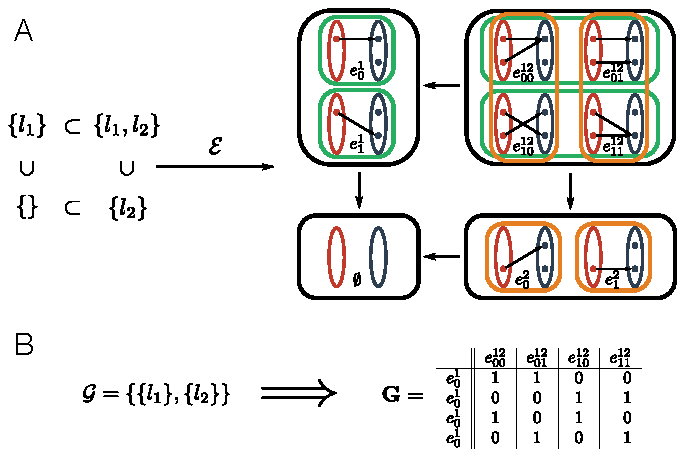
\includegraphics[width=0.8\columnwidth]{fig/efunctor.pdf}
\caption{{\bf Example of the functor mapping subsets of genes to measurable spaces.} (A) On the left hand side are subsets of $L=\{l_1,l_2\}$ ordered by inclusion. On the right hand side are the spaces of gene network-phenotype maps also ordered by inclusion. The labels for the maps define them. For example, $e^{12}_{01}(l_1) = 0$ and $e^{12}_{01}(l_2) = 1$. (B) For the given covering, $\mathcal{G}$, the associated marginalization matrix acting on the probability vector $\{ p^{12}_{00},p^{12}_{01},p^{12}_{10},p^{12}_{11} \}$ to give $\{ p^{1}_{0},p^{1}_{1},p^{2}_{0},p^{2}_{1} \}$ is $\mathbf{G}$.}
\label{fig:efunctor}
\end{figure}

\pagebreak

\begin{figure}[!ht]
\centering
\noindent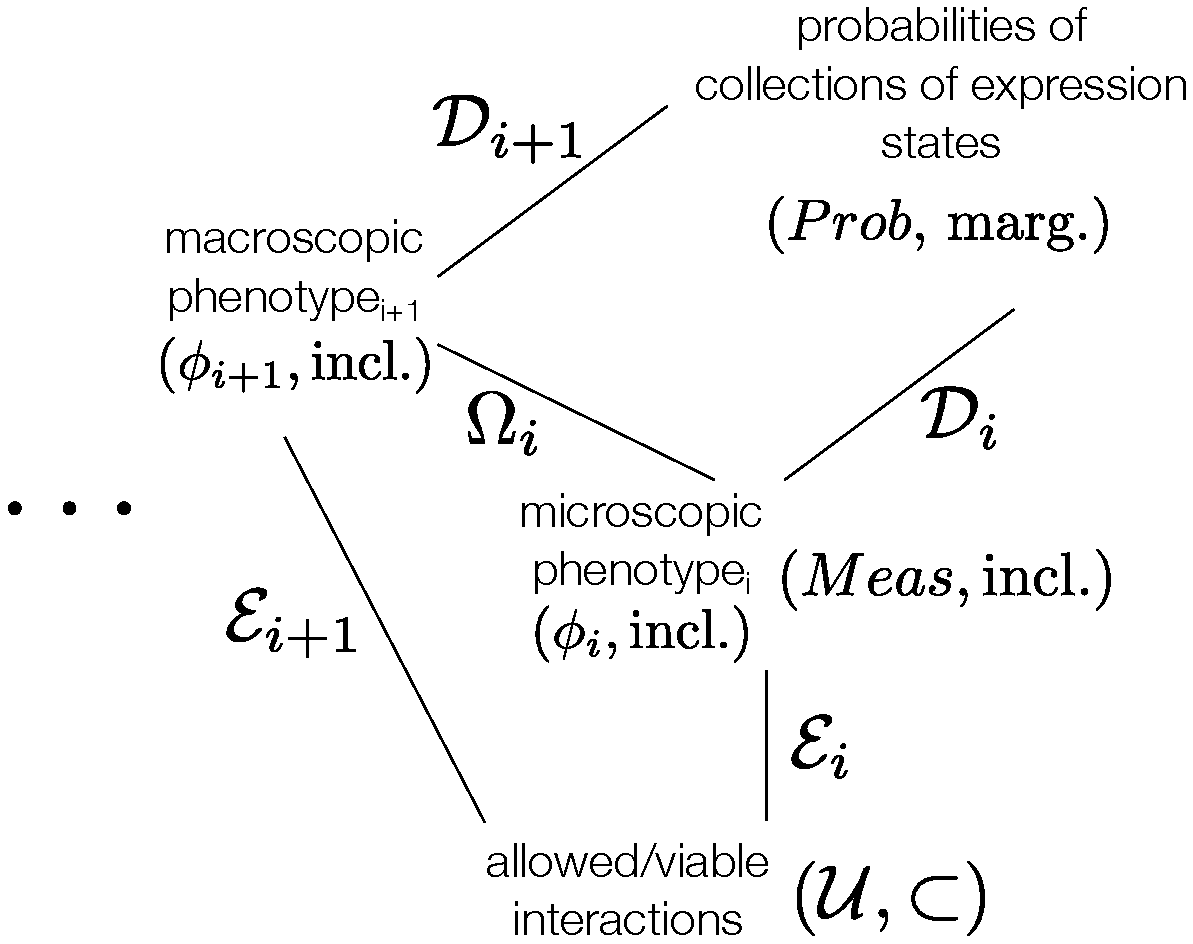
\includegraphics[width=0.4\columnwidth]{fig/abstractroadmap.pdf}
\caption{{\bf Mathematical relationships defining the hierarchy of phenotypes via coarse-graining.} }
\label{fig:abstractroadmap}
\DIFaddbeginFL \end{figure}

\pagebreak

\begin{figure}[!ht]
\centering
\noindent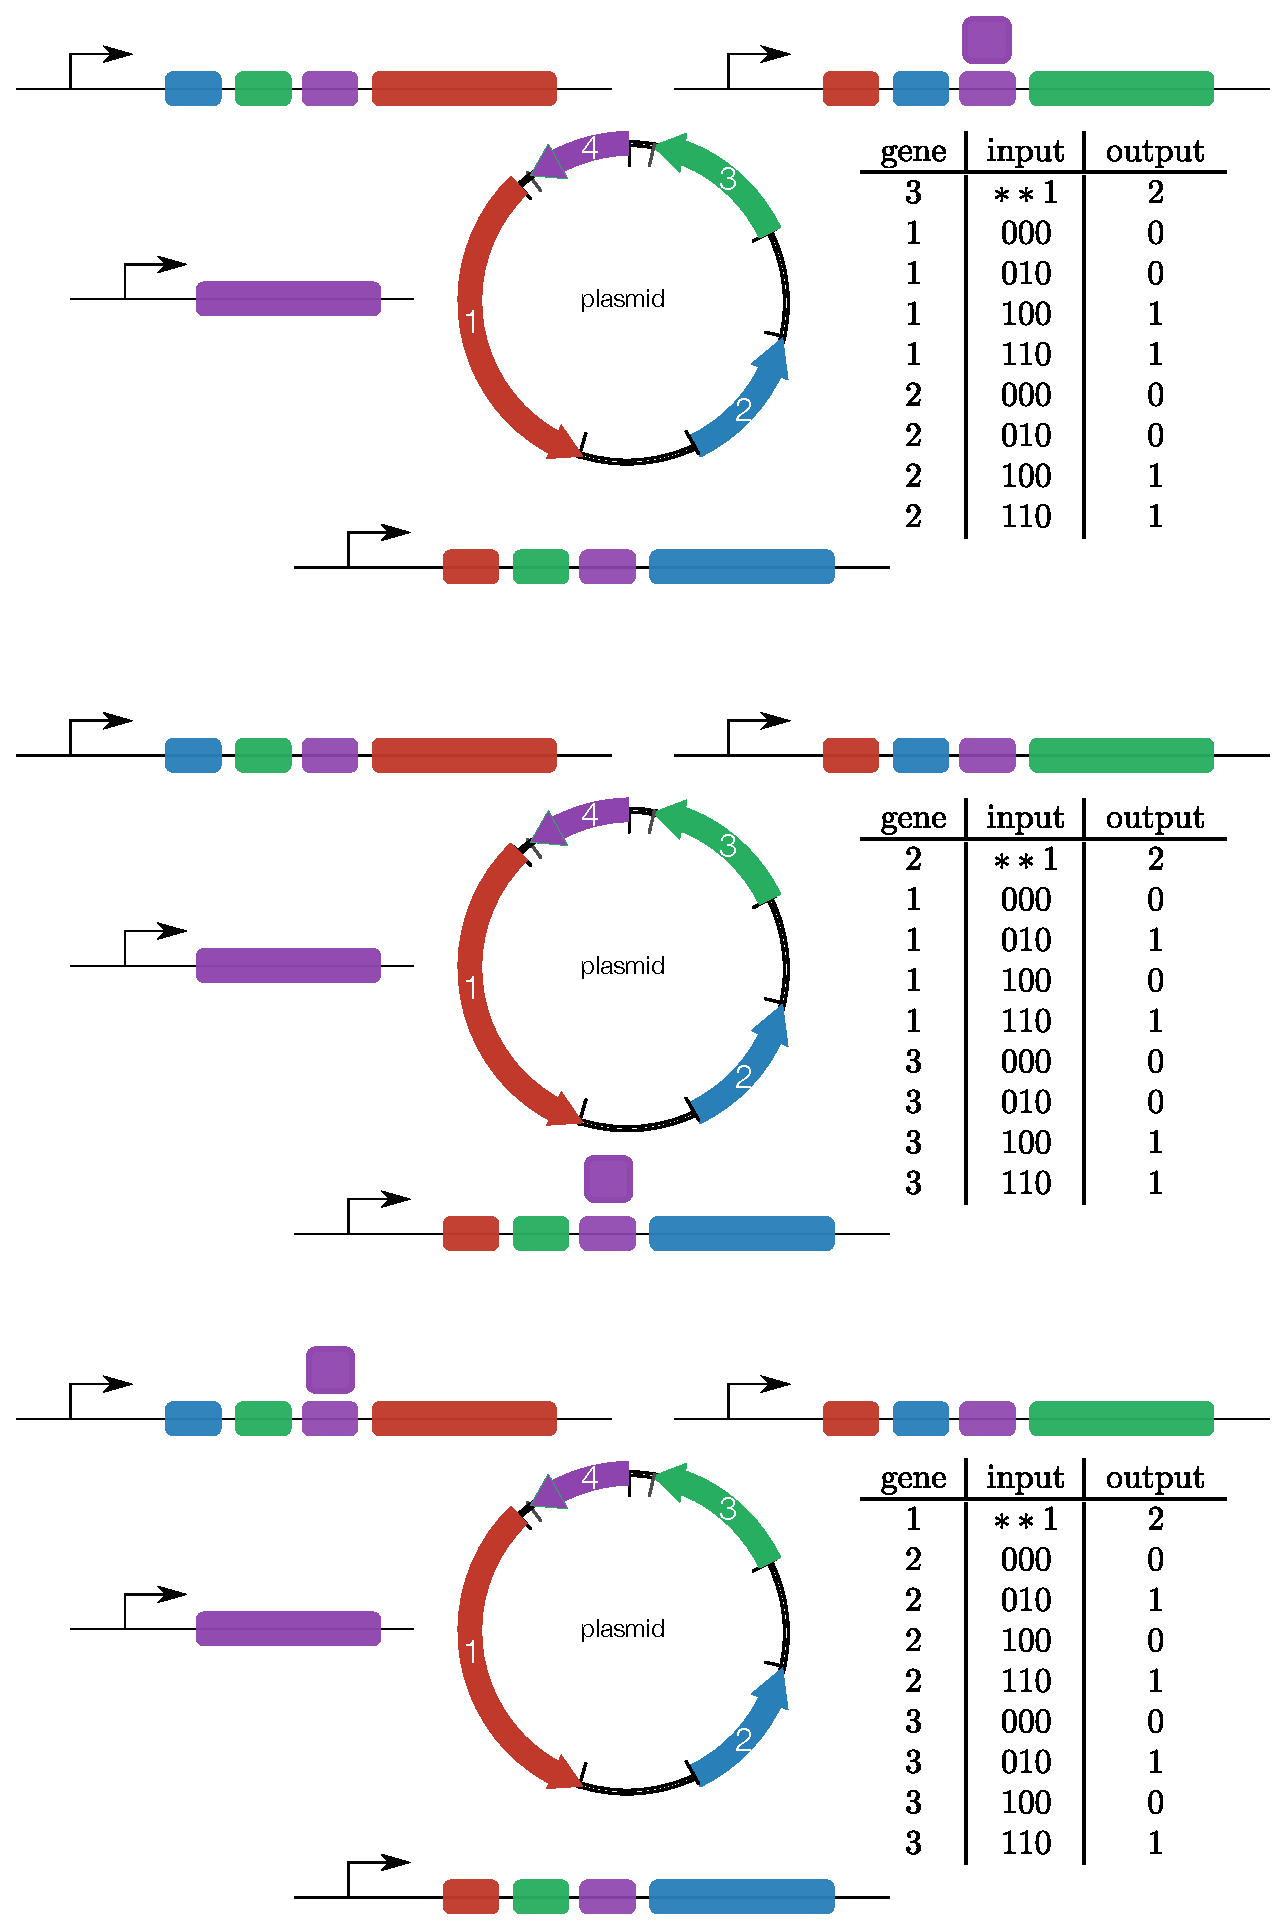
\includegraphics[width=1.0\columnwidth]{fig/condgenescenario.pdf}
\caption{{\bf \DIFaddFL{Schematic synthetic gene circuit capable of exhibiting apparent inconsistency.}} \DIFaddFL{A synthetic gene circuit consisting of four genes possesses one gene (purple) whose product is assumed to be present at low copy number and binds randomly with equal affinity to operator sites existing within the operons of each of the other three genes (red, blue, and green). These latter three genes each possess operator sites for the other two, but do not possess autoregulatory operators. They also each exhibit three states represented by three dynamical modes that may involve intermediates not explicitly represented here \mbox{%DIFAUXCMD
\cite{Cai2008,Dolmetsch1998}
}%DIFAUXCMD
. If the first gene is bound to the operator of another gene, the output is forced into a zero frequency infinite period, or DC, mode (state 2) regardless of the binding state of the other operators. If the first gene is unbound, then the expression state can be switched between low (state 0) and high (state 1) frequency modes depending upon the binding states of other genes as indicated. Note that operators for each of genes one to three are insensitive to the DC mode. Observing pairs of genes one to three and ignoring the state corresponding to the DC mode can lead to apparent inconsistency.}}
\label{fig:condgenescenario}
\DIFaddendFL \end{figure}



\pagebreak

\begin{figure}[!ht]
\centering
\noindent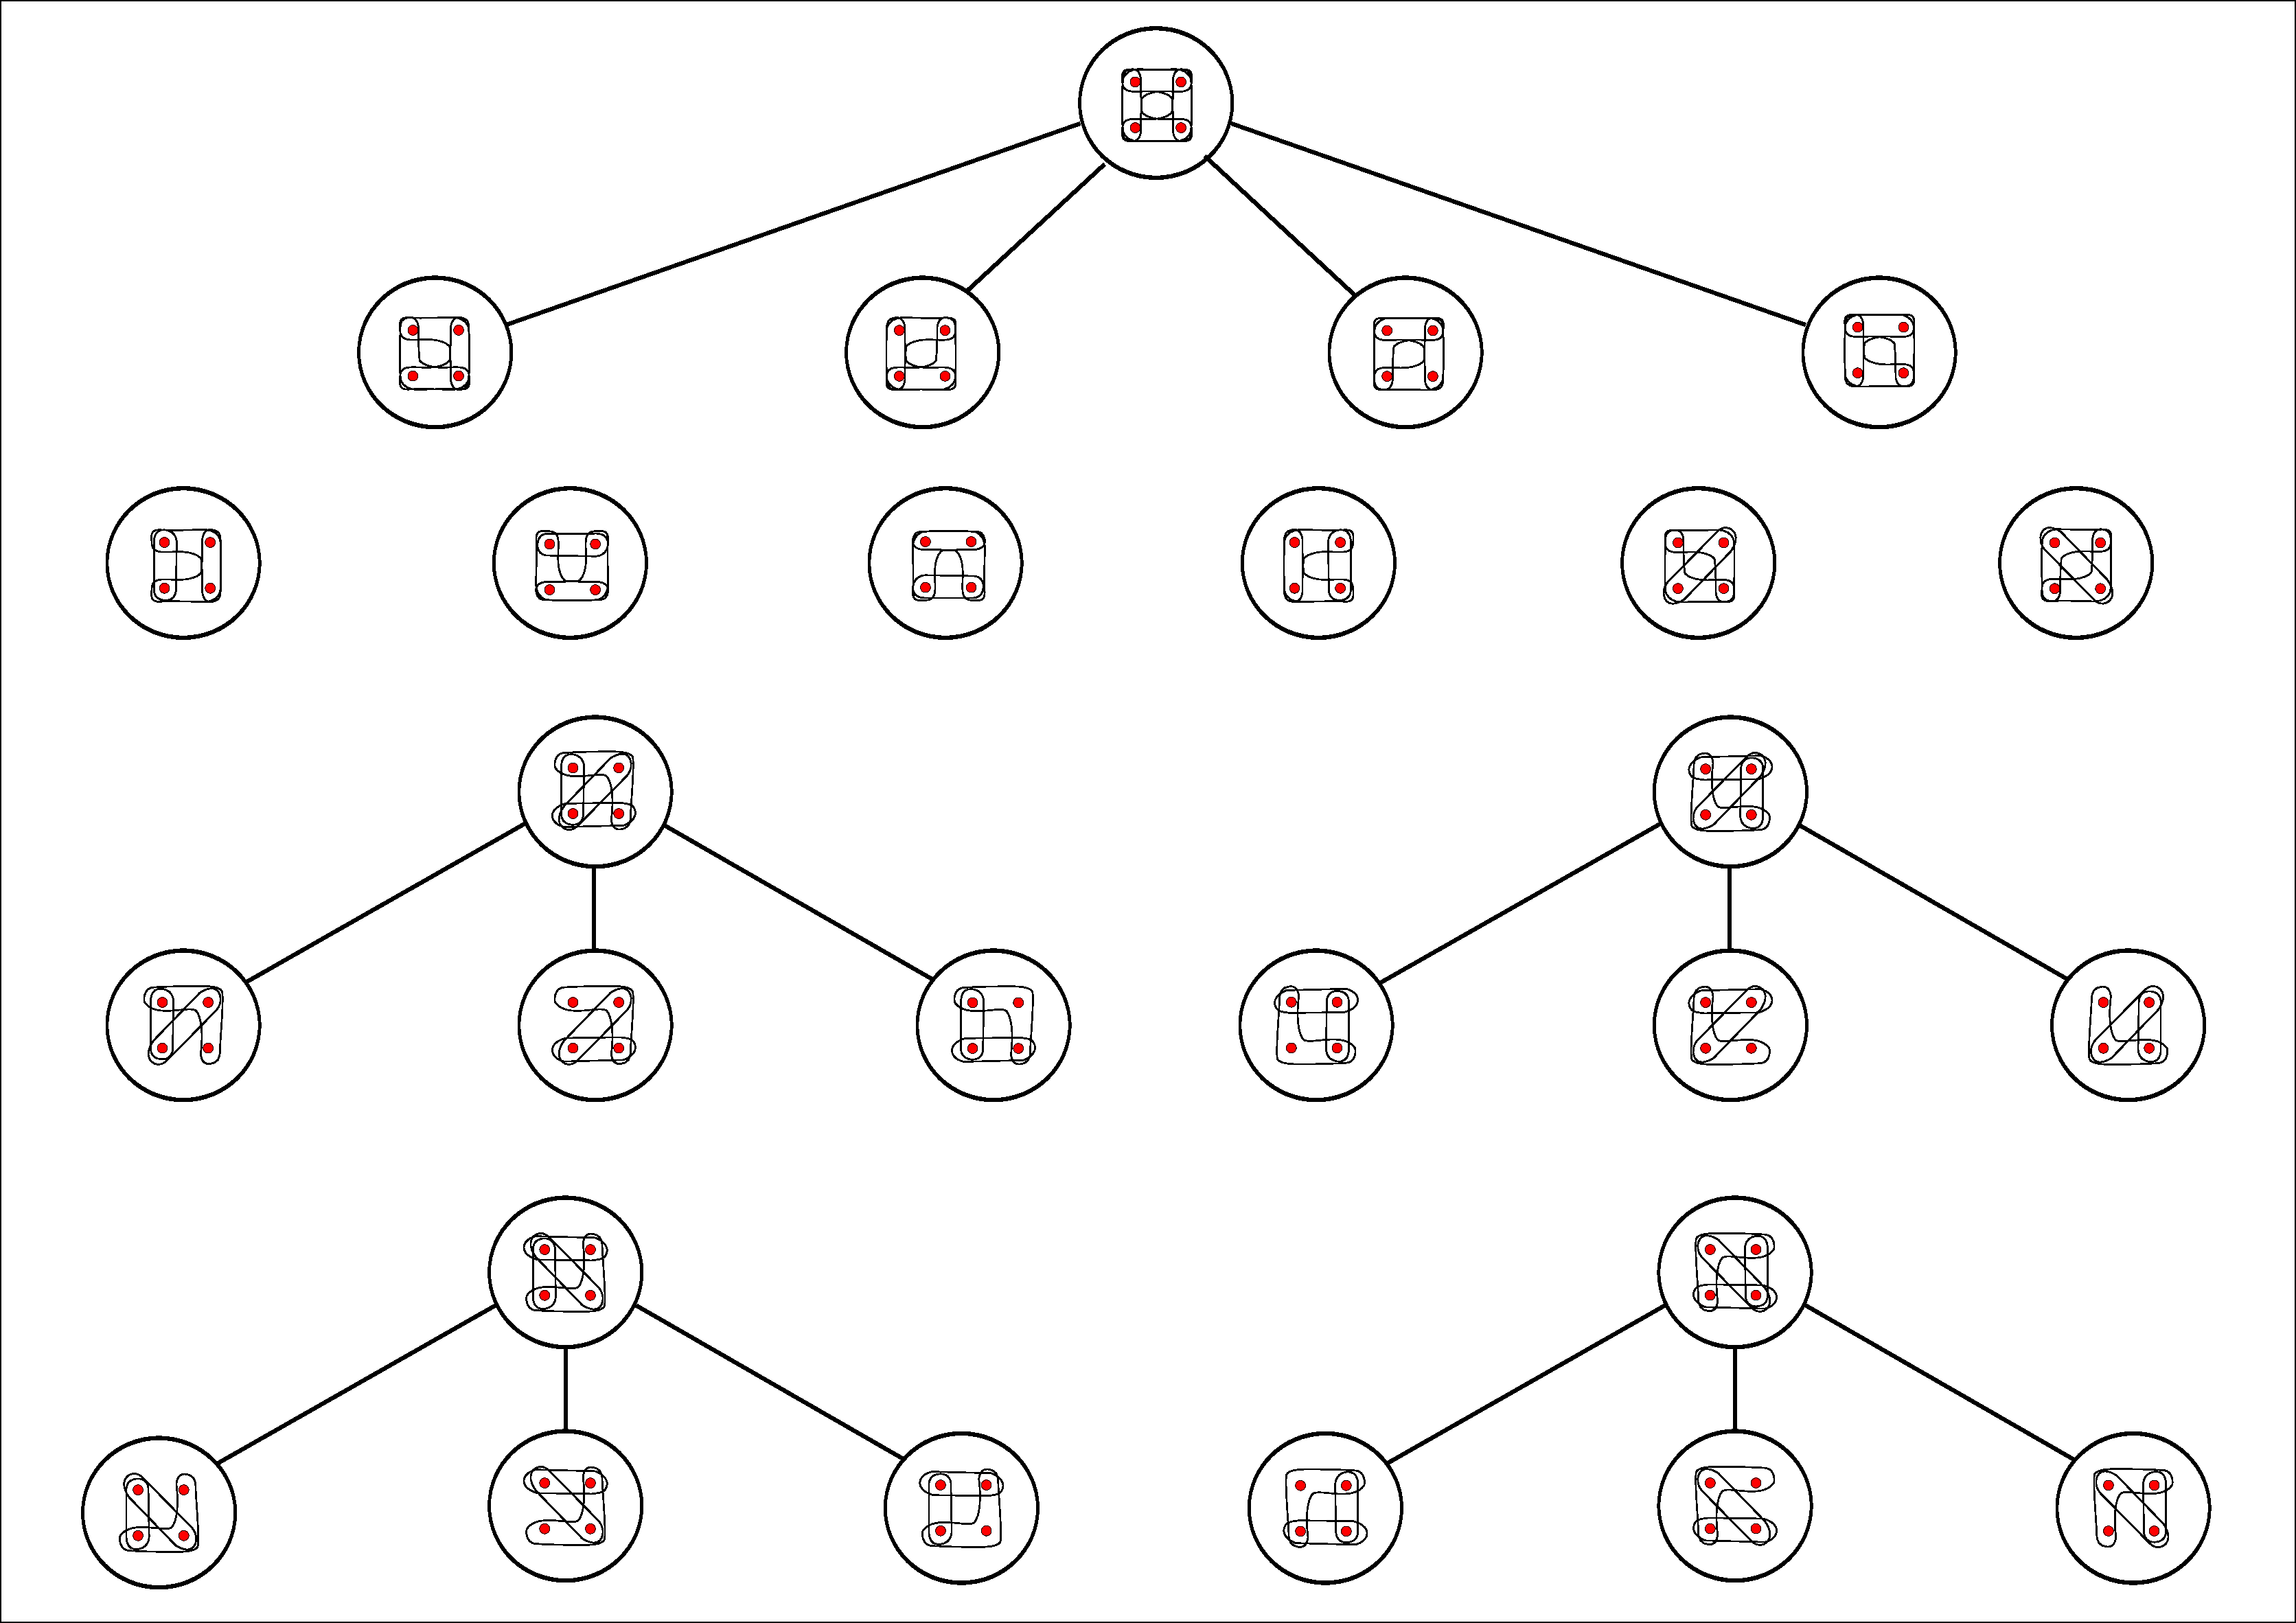
\includegraphics[width=1.0\columnwidth]{fig/non2uniformcyclichypergraphhasse.pdf}
\caption{{\bf Hierarchical relationships among all possible classes of hypergraphs that are not graphs (i.e. not 2-uniform) but have cycles.} (A) There is a Hasse diagram for the lattice of GRNAs analogous to that of \ref{fig:conediagram}A but defined on four rather than only three genes. Within this lattice some of the graphs have cycles and some do not. (B) The highest levels of the Hasse diagram associated to the lattice of GRNAs on four genes containing hypergraphs having cycles. (C) and (D) contain lower levels of GRNAs containing cycles. Each of the four panels in (D) are on the same level. In total, each level represents an isomorphism class of hypergraphs. Therefore, there are five isomorphism classes of non-2-uniform hypergraphs representing GRNAs on four genes that contain cycles leading to the relationship between spaces of probability distsributions on associated genotype-phentoype maps analogous to that of \ref{fig:conediagram}C.}
\label{fig:non2uniformcyclichypergraphhasse}
\end{figure}






\FloatBarrier
\pagebreak
\makeatletter{}\begin{table}[!ht]
\centering
\begin{tabular}{ r || c | c | c | c | c | c | c | c | c | c | c | c | c | c | c | c }
		 &	\begin{sideways}$e^{1234}_{0000}$\end{sideways} & \begin{sideways}$e^{1234}_{0010}$\end{sideways} & \begin{sideways}$e^{1234}_{0001}$\end{sideways} & \begin{sideways}$e^{1234}_{0011}$\end{sideways}
			  & \begin{sideways}$e^{1234}_{1000}$\end{sideways} & \begin{sideways}$e^{1234}_{1010}$\end{sideways} & \begin{sideways}$e^{1234}_{1001}$\end{sideways} & \begin{sideways}$e^{1234}_{1011}$\end{sideways}
			  &	\begin{sideways}$e^{1234}_{0100}$\end{sideways} & \begin{sideways}$e^{1234}_{0110}$\end{sideways} & \begin{sideways}$e^{1234}_{0101}$\end{sideways} & \begin{sideways}$e^{1234}_{0111}$\end{sideways}
			  &	\begin{sideways}$e^{1234}_{1100}$\end{sideways} & \begin{sideways}$e^{1234}_{1110}$\end{sideways} & \begin{sideways}$e^{1234}_{1101}$\end{sideways} & \begin{sideways}$e^{1234}_{1111}$\end{sideways}\\ \hline \hline
    $e^{12}_{00}$ & 1 & 1 & 1 & 1 & 0 & 0 & 0 & 0 & 0 & 0 & 0 & 0 & 0 & 0 & 0 & 0\\ \hline
    $e^{12}_{10}$ & 0 & 0 & 0 & 0 & 1 & 1 & 1 & 1 & 0 & 0 & 0 & 0 & 0 & 0 & 0 & 0\\ \hline
    $e^{12}_{01}$ & 0 & 0 & 0 & 0 & 0 & 0 & 0 & 0 & 1 & 1 & 1 & 1 &  0 & 0 & 0 & 0\\ \hline
    $e^{12}_{11}$ & 0 & 0 & 0 & 0 & 0 & 0 & 0 & 0 & 0 & 0 & 0 & 0 & 1 & 1 & 1 & 1\\ \hline

    $e^{32}_{00}$ & 1 & 0 & 1 & 0 & 1 & 0 & 1 & 0 & 0 & 0 & 0 & 0 & 0 & 0 & 0 & 0\\ \hline
    $e^{32}_{10}$ & 0 & 1 & 0 & 1 & 0 & 1 & 0 & 1 & 0 & 0 & 0 & 0 & 0 & 0 & 0 & 0\\ \hline
    $e^{32}_{01}$ & 0 & 0 & 0 & 0 & 0 & 0 & 0 & 0 & 1 & 0 & 1 & 0 & 1 & 0 & 1 & 0\\ \hline
    $e^{32}_{11}$ & 0 & 0 & 0 & 0 & 0 & 0 & 0 & 0 & 0 & 1 & 0 & 1 & 0 & 1 & 0 & 1\\ \hline

    $e^{14}_{00}$ & 1 & 1 & 0 & 0 & 0 & 0 & 0 & 0 & 1 & 1 & 0 & 0 & 0 & 0 & 0 & 0\\ \hline
    $e^{14}_{10}$ & 0 & 0 & 0 & 0 & 1 & 1 & 0 & 0 & 0 & 0 & 0 & 0 & 1 & 1 & 0 & 0\\ \hline
    $e^{14}_{01}$ & 0 & 0 & 1 & 1 & 0 & 0 & 0 & 0 & 0 & 0 & 1 & 1 & 0 & 0 & 0 & 0\\ \hline
    $e^{14}_{11}$ & 0 & 0 & 0 & 0 & 0 & 0 & 1 & 1 & 0 & 0 & 0 & 0 & 0 & 0 & 1 & 1\\ \hline

    $e^{34}_{00}$ & 1 & 0 & 0 & 0 & 1 & 0 & 0 & 0 & 1 & 0 & 0 & 0 & 1 & 0 & 0 & 0\\ \hline
    $e^{34}_{10}$ & 0 & 1 & 0 & 0 & 0 & 1 & 0 & 0 & 0 & 1 & 0 & 0 & 0 & 1 & 0 & 0\\ \hline
    $e^{34}_{01}$ & 0 & 0 & 1 & 0 & 0 & 0 & 1 & 0 & 0 & 0 & 1 & 0 & 0 & 0 & 1 & 0\\ \hline
    $e^{34}_{11}$ & 0 & 0 & 0 & 1 & 0 & 0 & 0 & 1 & 0 & 0 & 0 & 1 & 0 & 0 & 0 & 1\\
    \end{tabular}
\caption{Explicit construction of $\mathbf{G}_{n \times m}$ for the case $L = \{ l_1,l_2,l_3,l_4 \}$, $\mathcal{G} = \{\{l_1,l_2 \},\{l_1,l_4 \},\{l_3,l_2\},\{l_3,l_4\} \}$, $P=\{0,1\}$ and thus $\mathbf{G}_{(2 \cdot 2)^2 \times 2^{2 \cdot 2}} = \mathbf{G}_{16 \times 16}$.}
\label{tab:logmat222}
\end{table}


\FloatBarrier
\pagebreak


\end{document}
